% Nejprve uvedeme tridu dokumentu s volbami
\documentclass[czech,bachelor]{diploma}
% Dalsi doplnujici baliky maker
\usepackage[autostyle=true,czech=quotes]{csquotes} % korektni sazba uvozovek, podpora pro balik biblatex
\usepackage[backend=biber, style=iso-numeric, alldates=iso]{biblatex} 
\let\biblatexaddspace\addspace

\usepackage{dcolumn} % sloupce tabulky s ciselnymi hodnotami
\usepackage{subfig} % makra pro "podobrazky" a "podtabulky"
\usepackage[cpp]{diplomalst}

\usepackage{float}
\usepackage{threeparttable}
\usepackage{fontawesome}
%\usepackage{todonotes}
\usepackage{comment}
\usepackage[miktex]{gnuplottex}
\usepackage{imakeidx}
\usepackage{graphicx}
\usepackage{musixtex}
\usepackage{courier}
\usepackage{lmodern}

\makeindex[columns=1, title=Alphabetical Index, intoc]

% Zadame pozadovane vstupy pro generovani titulnich stran.
\ThesisAuthor{Josef Micak}

\ThesisSupervisor{doc. Mgr. Jiří Dvorský, Ph.D.}

\CzechThesisTitle{Čínská dáma}

\EnglishThesisTitle{Chinese Checkers}

\SubmissionYear{2021}

% Pokud nechceme nikomu dekovat makro zapoznamkujeme.
\Acknowledgement{Chtěl bych tímto poděkovat vedoucímu mé bakalářské práce, doc. Mgr. Jiřímu Dvorskému, Ph.D. za poskytnutí konstruktivních poznatků k obsahu práce a za trpělivost a čas strávený při konzultacích týkajících se této práce.}

\CzechAbstract{Cílem této bakalářské práce je implementovat počítačovou podobu deskové hry Čínská dáma. K~implementaci hry je využíván programovací jazyk C\#, je umožněna hra člověka proti dvěma až pěti počítačovým hráčům. Další části bakalářské práce obsahují popis této deskové hry a~analýzu množství ukázkových partií.}

\CzechKeywords{Bakalářská práce; Čínská dáma; C\#; programování; desková hra}

\EnglishAbstract{The purpose of this bachelor thesis is to implement the computer form of the board game Chinese Checkers. The C\# programming language is used for implementation purposes, the implementation supports playing against two to five computer opponents. Other parts of the thesis include description of this board game and analysis of a number of exemplary games.}

\EnglishKeywords{Bachelor thesis; Chinese Checkers; C\#; programming; board game}

\addbibresource{MyB.bib}

\makeatletter
\newcommand*{\mxaddspace}[1]{\kern#1\global\advance\x@skip#1}
\makeatother

% Novy druh tabulkoveho sloupce, ve kterem jsou cisla zarovnana podle desetinne carky
\newcolumntype{d}[1]{D{,}{,}{#1}}

% Zacatek dokumentu
\begin{document}

% Nechame vysazet titulni strany.
\MakeTitlePages

% A nasleduje text zaverecne prace.
\chapter{Úvod}
\label{sec:Introduction}
Tato bakalářská práce se zabývá deskovou hrou \emph{Čínská dáma}. Ačkoli by tomu název mohl napovídat, tato hra toho nemá příliš společného s mnohem známější hrou, kterou známe pod názvem Dáma. Navíc existuje více interpretací pravidel, týkajících se počtu herních polí a kamenů hráče, nebo samotných tahů. Nejprve je tedy čtenář seznámen s důležitými teoretickými podklady týkajícími se hry –- původem hry, principem hry a zvoleným souborem pravidel. Následuje objektová analýza hry, ze které se vychází při samotné implementaci.

Cílem práce je lidskému hráči umožnit odehrání hry proti jednomu až pěti počítačovým hráčům nastavitelných obtížností. Práce zahrnuje popis jednotlivých obtížností počítačového hráče a~v~samotné hře je implementován simulátor, ve kterém si lidský hráč může nasimulovat hru mezi volitelným počtem počítačových hráčů volitelných obtížností a sledovat průběh hry a její výsledek. Pro praktickou ukázku chování nepřátel podle jejich obtížností práce obsahuje analýzu většího množství her mezi počítačovými hráči stejných i různých obtížností.
\endinput
\chapter{Teoretické podklady}
\section{Původ hry}
Čínská dáma má velmi zavádějící název \cite{puvod-cz}. Nepochází z Číny, ale pravděpodobně z Německa nebo Švédska, a s Dámou nemá také v podstatě nic společného. Je velmi podobná Halmě. 

Právě k Halmě může být původ Čínské dámy vysledován \cite{puvod-en}. Jedná se o hru, která byla populární ve Velké Británii v 70. letech 19. století, a která byla založena na starší britské deskové hře zvané \enquote{Hoppity}. Šesticípá hvězda neboli \enquote{Stern} byla v deskové podobě představena v roce 1892 německou herní společností Ravensburger, která hru pojmenovala \enquote{Stern-Halma}. Později, v roce 1928, v~návaznosti na tehdejší světový zájem o orientální mystiku, jako například představení hry Mah Jong v roce 1923 a objevení hrobky krále Tutanchamona v roce 1922, J.~Pressman \& Co. pojmenoval tuto hru \enquote{Čínská dáma}. Hra byla na vrcholku popularity v Americe v 30.\ letech 20.\ století. I přes svou popularitu nebyla ale její minulost zcela zapomenuta, a v Německu, kde se jí stále říká Halma, se hraje podle původních pravidel.

\section{Princip a rozložení hry}
Herní deska Čínské dámy má tvar šesticípé hvězdy \cite{pravidla}. Každý cíp hvězdy je trojúhelník obsahující deset polí (z každé strany je hranice trojúhelníku tvořena čtyřmi poli). Vnitřek desky je hexagon, u něhož je z každé strany jeho hranice tvořena pěti poli. Každý trojúhelník má odlišné zabarvení a~k~dispozici je deset kamenů s odpovídajícími barvami.

Čínská dáma může být hrána dvěma, třemi, čtyřmi nebo šesti hráči \cite{pravidla}. U verze pro šest hráčů budou samozřejmě využity všechny kameny a trojúhelníky. U verze pro čtyři hráče začínají hráči ve dvou párech protilehlých cípů hvězdy, stejně tak u verze pro dva hráče by hráči měli začínat ze dvou protilehlých cípů. U verze pro tři hráče jsou kameny hráčů rozmístěny do tří spolu nesousedících trojúhelníků. Čínská dáma nemůže být hrána pěti hráči \cite{pravidla2}, protože by při takovém počtu hráčů jeden z hráčů bojoval proti prázdné straně hvězdy. Ukázkové počáteční rozložení kamenů na herní desce pro všechny dostupné počty hráčů je možno vidět na obrázku číslo \ref{fig:PocatecniRozlozeni}.

Cílem hry je být prvním hráčem, kterému se podaří přesunout všechny své kameny přes celou herní desku a umístit je do protilehlého cípu \cite{pravidla}. První hráč, kterému se povede obsadit všech deset polí v protilehlém cípu hvězdy, vyhrává. V případě, že více hráčů obsadí protilehlé cípy během stejného tahu, dochází k remíze.

\begin{figure}
	\centering
	\subfloat[2 hráči\label{fig:PocatecniRozlozeni2Hraci}]
	{
		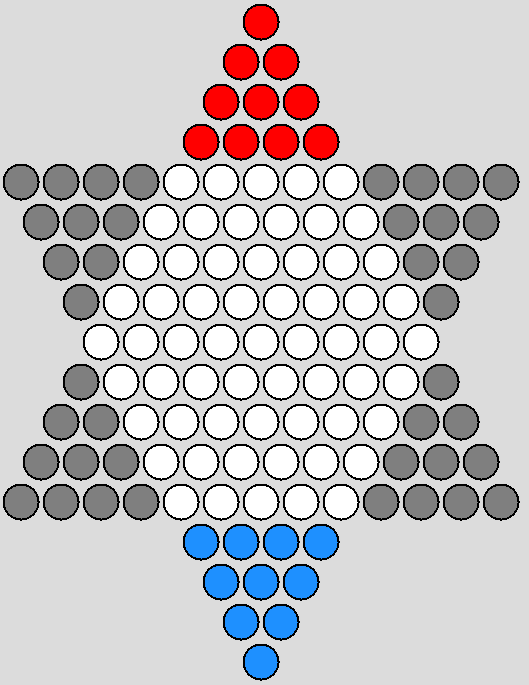
\includegraphics[width=0.35\textwidth]{Figures/PocatecniRozlozeni2Hraci.png}
	}
	\hspace{3em} % make more space
	\subfloat[3 hráči\label{fig:PocatecniRozlozeni3Hraci}]
	{
		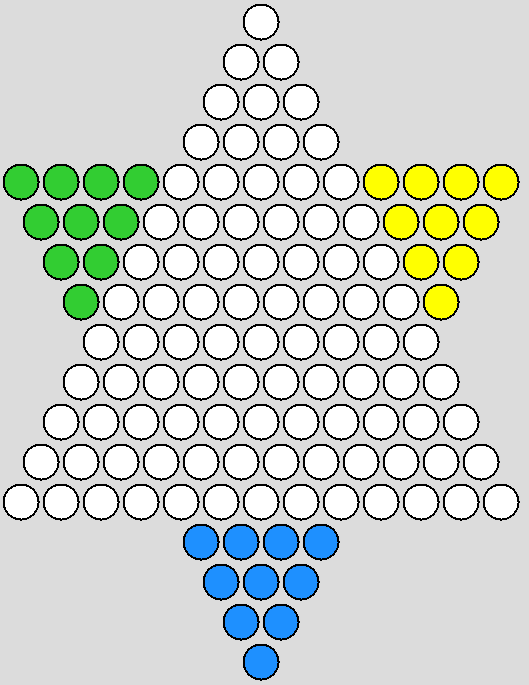
\includegraphics[width=0.35\textwidth]{Figures/PocatecniRozlozeni3Hraci.png}
	}
	\hspace{3em} % make more space
	\subfloat[4 hráči\label{fig:PocatecniRozlozeni4Hraci}]
	{
		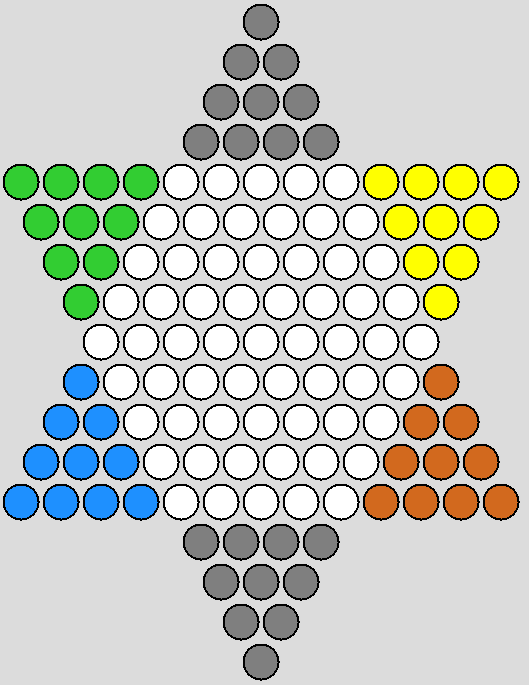
\includegraphics[width=0.35\textwidth]{Figures/PocatecniRozlozeni4Hraci.png}
	}
	\hspace{3em} % make more space
	\subfloat[6 hráčů\label{fig:PocatecniRozlozeni6Hracu}]
	{
		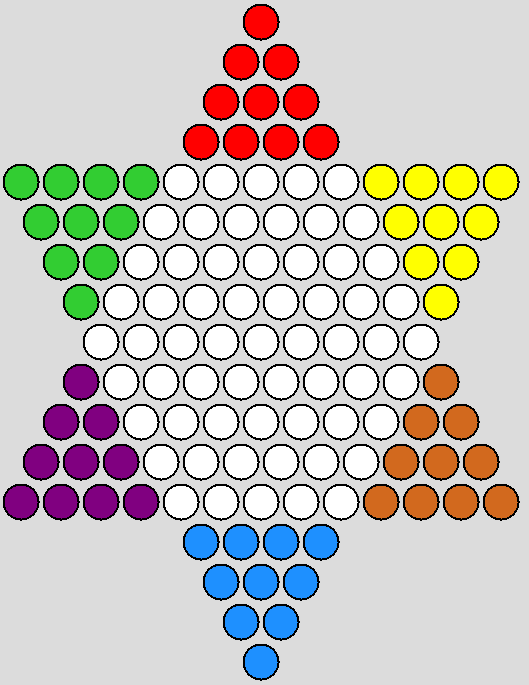
\includegraphics[width=0.35\textwidth]{Figures/PocatecniRozlozeni6Hracu.png}
	}
	\caption[Počáteční rozložení pro všechny dostupné počty hráčů]{Počáteční rozložení pro všechny dostupné počty hráčů (tmavě šedou barvou jsou vyznačena zablokovaná pole)}
	\label{fig:PocatecniRozlozeni}
\end{figure}

\section{Pravidla hry a jejich možné interpretace}
Ohledně pravidel a samotném rozložení hry nepanuje jasná shoda. Jak teoretické popisy, tak praktické implementace hry se od sebe navzájem velmi často liší. Rozdíly mezi jednotlivými verzemi hry jsou sice často pouze v detailech, mnohdy se ale verze hry navzájem liší v důležitých věcech, které zásadním způsobem ovlivňují průběh i výsledek hry. Tato sekce tedy kromě pravidel využívaných ve výsledné implementaci popisuje i další možné interpretace pravidel, se kterými je možné se setkat v dalších popisech a implementacích této hry.

Hráči se mohou mezi sebou dohodnout o tom, kdo z nich bude na tahu jako první \cite{pravidla2}. Pokud se hráči nechtějí o začínajícím hráči dohodnout mezi sebou, je hod mincí jedinou metodou zmíněnou v pravidlech sloužící k ustanovení začínajícího hráče. Následně se hráči v tazích střídají ve směru hodinových ručiček.

Během jednoho tahu přesouvá hráč vždy jediný kámen své barvy. Tyto kameny nelze během průběhu hry žádným způsobem vyřadit ze hry, všechny zůstávají po celou dobu hry na herní desce (na rozdíl od klasické Dámy nebo například šachů, kde k vyřazování kamenů nebo figurek hráčů naopak dochází).

Některé verze pravidel ustanovují, že hráči mohou ovládat více sad kamenů zároveň \cite{pravidla3}. Taková hra je umožněna za předpokladu, že jsou kameny v takovém rozložení, v jakém jsou v naší aplikaci při hře čtyř nebo šesti hráčů. Každý hráč pak ovládá dvě, resp. tři sady kamenů. Vyhrává ten hráč, který jako první přesune všechny své sady kamenů do daných protilehlých trojúhelníků. V rámci této práce má hráč k dispozici vždy jednu sadu kamenů.

Pravidla nejsou jednotná v povolených tazích, podle některých interpretací je možné vždy táhnout na kterékoli pole na desce, podle jiných je možné táhnout pouze na středový hexagon a na výchozí a protilehlý trojúhelník. V této práci byla zvolena varianta pravidel zakazující tahy na hráčské trojúhelníky s výjimkou výchozího trojúhelníku a protilehlého trojúhelníku daného hráče, a to při libovolném počtu hráčů. Zablokovaná (nebo můžeme říct také neaktivní) pole jsou vyznačena tmavě šedou barvou, jejich polohu můžeme vidět na obrázku číslo \ref{fig:PocatecniRozlozeni}.

Vždy panovaly nejasnosti ohledně situace, kdy hráč nemůže vyhrát, protože kámen hráče začínajícího v protilehlém cípu blokuje jedno z polí v daném cípu \cite{pravidla}. Mnohé verze pravidel žádný postup v takové situaci nezmiňují, což by se dalo pochopit tak, že je blokování soupeře tímto pochybným způsobem povoleno. Zde je tato situace vyřešena kontumační výhrou pro blokovaného hráče -- pokud hráč přemístí své kameny do všech volných polí protilehlého cípu a obsadit ta zbývající nemůže výhradně z důvodu, že jsou blokována nepřítelem, je mu udělena kontumační výhra. Tato situace nastává nejčastěji při výrazném dovednostním rozdílu mezi protilehlými hráči, kdy je jeden hráč schopen téměř dokončit hru dříve, než je druhý hráč schopen opustit svůj výchozí trojúhelník. Při testování programu vytvořeného v rámci této práce může tato situace nastat zejména v případě, že jsou do protilehlých cípů proti sobě postaveni počítačoví hráči protipólních obtížností.

Některé interpretace pravidel určují barvy hráčů podle výchozích trojúhelníků hráčů \cite{zapletal}. V této práci má pro přehlednost lidský hráč vždy modrou barvu, nezávisle na tom, který trojúhelník je jeho výchozím. Barvy jednotlivých hráčů budou také přiděleny s ohledem na co nejvyšší vzájemnou odlišitelnost, a to zejména kvůli tomu, že na desce je při každém tahu světlejším odstínem dané barvy vyznačeno pole, ze kterého během tahu daný hráč přesunul kámen.

\section{Možné tahy}
\label{sec:MozneTahy}
Během tahu může hráč kámen přesunout na sousední pole, nebo může provést jeden nebo více skoků přes ostatní kameny \cite{pravidla}. Skok musí být proveden do volného pole, které je za přeskakovaným kamenem, jinak řečeno, musíme být schopni vytvořit jedinou úsečku spojující přesouvaný kámen, přeskakovaný kámen a volné pole, na které chceme doskočit. Každý skok může být proveden přes jakýkoli kámen na herní desce včetně vlastních kamenů. Po každém skoku může hráč buď tah hned ukončit, nebo může pokračovat skokem přes další kámen. Během hry tedy může nastat situace, při které hráč může přesunout kámen z výchozího do protilehlého trojúhelníku v jediném tahu.

Když hráč provádí skok, nesmí být mezi přeskakovaným a přesouvaným kamenem žádný jiný kámen, nelze tedy přeskočit dva a více kamenů během jednoho skoku. Vzdálenost mezi přesouvaným kamenem a přeskakovaným kamenem se musí rovnat vzdálenosti mezi přeskakovaným kamenem a~volným polem, na které chceme doskočit. Mnohé verze pravidel taktéž zmiňují, že po provedení prvního skoku musí být všechny další skoky v rámci daného tahu právě tak dlouhé jako první skok. Na toto pravidlo je při implementaci této práce brán zřetel, délka skoků se tedy v rámci jednoho tahu nemůže lišit.

Zásadní věc, ve které se různé verze pravidel od sebe odlišují, jsou povolené směry tahů. Z~pohledu na herní desku lze určit, že tah lze provést celkem šesti směry (viz obrázek číslo \ref{fig:MozneTahy - Sousedni}). Podle některých názorů je ale zakázáno provádět tahy dozadu, tedy směrem k výchozímu trojúhelníku, což ve výsledku omezí počet povolených směrů na čtyři. V rámci této práce je na toto omezení brán zřetel, a hráči se tak mohou pohybovat všemi šesti směry.

\begin{figure}
	\centering
	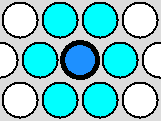
\includegraphics[width=0.4\textwidth]{Figures/MozneTahy - Sousedni.png}
	\caption[Sousední pole, na která je možný přesun]{Sousední pole, na která je možný přesun -- vyznačena světle modře}
    \label{fig:MozneTahy - Sousedni}
\end{figure}

Pro lepší pochopení možných tahů je k dispozici vyobrazení volných polí, na která se hráč může přesunout, zahrnující jak přesuny na sousední pole, tak skoky s různou vzdáleností, na obrázku číslo~\ref{fig:MozneTahy - Skoky}.

\begin{figure}
	\centering
	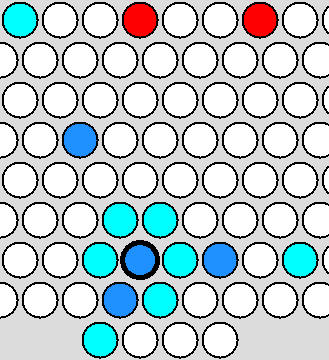
\includegraphics[width=0.4\textwidth]{Figures/MozneTahy - Skoky.png}
	\caption[Pole, na která je možno se přesunout nebo skočit]{Pole, na která je možno se přesunout nebo skočit -- vyznačena světle modře}
    \label{fig:MozneTahy - Skoky}
\end{figure}

\section{Strategie}
\label{sec:Strategie}
Čínská dáma je strategická hra \cite{strategie}, a během její existence tak vymysleli hráči množství strategií, použitelných ve všech fázích hry, jejichž cílem je co nejefektivnější a nejrychlejší přesun všech kamenů do protilehlého trojúhelníku.

Dva nejpoužívanější prvotní tahy jsou Sidewinder a Cross Caterpillar \cite{strategie}. Sidewinder spočívá v~přesunu dvou kamenů nejvzdálenějších od cípu trojúhelníku diagonálně směrem pryč od trojúhelníku. Tato strategie umožní pohyb přes neočekávaná místa, zatímco jiné, často užívané strategie provádějí pohyb přes střed herní desky.

\begin{figure}
	\centering
	\subfloat[tah Sidewinder\label{fig:TahSidewinder}]
	{
		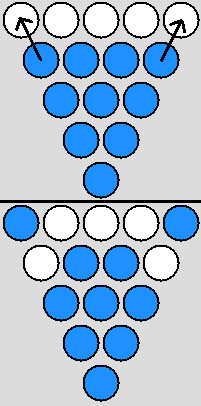
\includegraphics[width=0.35\textwidth]{Figures/PrvotniTahSidewinder.png}
	}
	\hspace{3em} % make more space
	\subfloat[tah Cross Caterpillar\label{fig:TahCrossCaterpillar}]
	{
		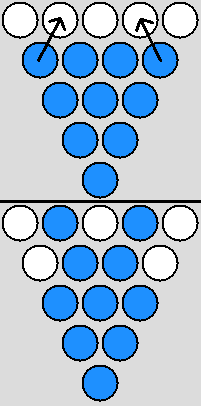
\includegraphics[width=0.35\textwidth]{Figures/PrvotniTahCrossCaterpillar.png}
	}
	\caption{Porovnání nejpoužívanějších prvotních tahů -- Sidewinder a Cross Caterpillar}
	\label{fig:PrvotniTahy}
\end{figure}

Dalším často používaným prvotním tahem je Cross Caterpillar \cite{strategie}. Ten je podobný tahu Sidewinder, s tím rozdílem, že namísto pohybu směrem pryč od trojúhelníku je pohyb proveden směrem ke středu trojúhelníku. Oba tyto tahy jsou velmi efektivní a slouží jako dobrý základ pro další strategické tahy. Porovnání těchto dvou tahů je na obrázku číslo \ref{fig:PrvotniTahy}.

Po provedení prvotních tahů jsou na řadě strategie zaměřené na zbytek hry. Zde jistě stojí za zmínku taktika shlukování \cite{strategie}. Ta je založená na principu vedení kamenů blízko u sebe. Jinak řečeno, hráčovy kameny se přesouvají spolu jako jeden celek, ne jako malé, oddělené skupinky kamenů. Použití této strategie donutí nepřítele k nasměrování svých pohybů kolem kamenů hráče, který tuto taktiku používá. To ve výsledku zpomalí nepřítelův postup, zatímco hráč se postupně stále přibližuje k protilehlému cípu.

Další strategií je blokování \cite{strategie2}. Podle této strategie je nutné neklást důraz pouze na nejvyšší možnou vzdálenost, kterou je možné s kamenem během jednoho tahu urazit, nýbrž je někdy možné získat větší výhodu zablokováním soupeře, a to bez ohledu na vzdálenost mezi kamenem a cílovým polem. Mnohdy je takto nazýváno úmyslné ponechání kamene ve výchozím trojúhelníku, což ve výsledku znemožní hráči z protilehlého cípu dokončit hru. Této taktice se také říká \enquote{spoiling} a je obecně považována za pochybnou.

Strategií určenou pro středovou fázi hry je postavení mostu \cite{strategie}. Tento most umožní hráči efektivně přesouvat kameny z jednoho konce desky na druhý. Je ale nutné mít na paměti, že nepřítel bude také mít možnost využívat tento most. Je proto nutné se proti této možnosti bránit například využitím blokování. Na obrázku číslo \ref{fig:Most} je k nahlédnutí ukázka jednoduchého mostu, který může být vybudován během čtyř tahů.

\begin{figure}
	\centering
	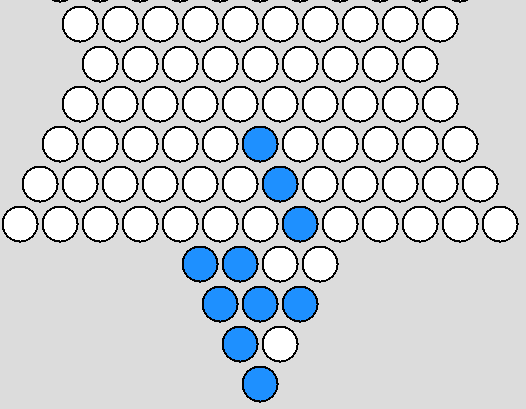
\includegraphics[width=0.4\textwidth]{Figures/Most.png}
	\caption{Ukázka strategie postavení mostu}
    \label{fig:Most}
\end{figure}

V závěrečné fázi hry, kdy hráč začne obsazovat protilehlý trojúhelník, je výhodné nejprve obsadit hrany tohoto pomyslného trojúhelníku \cite{strategie2}, a až poté jeho středové části. Tento postup mírně ulehčí přesunutí zbývajících kamenů do cílového trojúhelníku.
\endinput
\chapter{Rozbor hry}
\section{Herní deska}
Herní deska má vždy tvar šesticípé hvězdy, nezávisle na počtu hráčů. Existují dvě verze desek, lišící se v počtu herních polí a kamenů přidělovaných hráčům. Podle jedné verze by měla deska obsahovat celkem 192 polí \cite{zapletal}, s tím že každému hráči je přiděleno patnáct kamenů (s výjimkou případu, kdy probíhá hra šesti hráčů, v takovém případě zůstává nejdelší řada ve výchozím trojúhelníku hráče prázdná a každý hráč má tedy pouze deset kamenů). Herní desku v této verzi můžeme vidět na obrázku číslo \ref{fig:VerzeHerniDesky}.

\begin{figure}
	\centering
	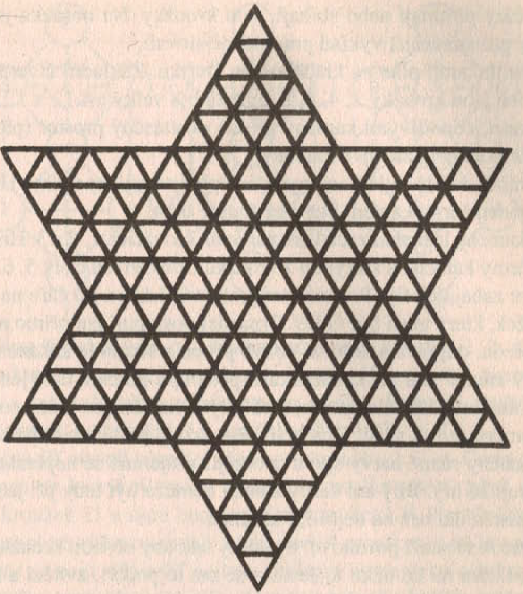
\includegraphics[width=0.4\textwidth]{Figures/VerzeHerniDesky.png}
	\caption{Verze herní desky obsahující 192 polí \cite{zapletal}}
    \label{fig:VerzeHerniDesky}
\end{figure}

Zmíněná verze herní desky již ale není v dnešní době příliš používána. I v této práci je využita druhá verze desky, ve které je obsaženo 121 polí, a každému hráči je přiděleno bez ohledu na počet hráčů vždy deset kamenů. Tato herní deska obsahuje 17 sloupců a 13 řádků. U žádných dvou sousedních polí na desce nelze vytvořit vertikální úsečku spojující jejich středy -– každé pole je totiž horizontálně umístěno přesně mezi pole nalézající se nad ním nebo pod ním. Vytvoření horizontálních úseček spojující středy dvou sousedních polí je oproti tomu umožněno. Samotná herní deska je~v~naší aplikaci uložena v okně \lstinline$HraForm$ v panelu pojmenovaném \lstinline$herniPanel$. Ten slouží k práci s~vytvořenými herními poli.

\section{Herní pole}
\label{sec:HerniPole}
Jako první je vytvořeno pole nalézající se z pohledu uživatele na samotném vrcholu trojúhelníku, jedná se o pole s nejnižší $y$-ovou souřadnicí ze všech polí. U tohoto pole bylo zvoleno vhodné odsazení od hranic panelu, vzorec pro určení odsazení na $x$-ové ose je uveden v rovnici (\ref{eq:leveOdsazeni}), na $y$-ové je rovno hodnotě 13px. Poloha všech ostatních polí se odvíjí od tohoto pole, protože poloha každého pole je přímo závislá na poloze předchozího vytvořeného pole.

\begin{equation}
leveOdsazeni = \frac{1}{2}(sirkaPanelu - sirkaPole)
\label{eq:leveOdsazeni}
\end{equation}

$X$-ová a $y$-ová souřadnice daného pole jsou uloženy v proměnných \lstinline$poz_X_He$ a \lstinline$poz_Y_He$. Mezi další parametry každého pole patří jeho šířka a výška, ty jsou uloženy v proměnných \lstinline$sirkaPole$~a~\lstinline$vyskaPole$ a jejich hodnota činí 35px. Mezi všemi poli je ve všech směrech rozestup o hodnotě 5px, pro usnadnění je proto vytvořená proměnná \lstinline$posun$ označující vzdálenost mezi dvěma sousedními poli, a to horizontálně i vertikálně, rovnající se součtu rozměru pole a rozestupu mezi poli, tedy 40px. Znázornění souřadnic všech polí je k dispozici na obrázku číslo \ref{fig:SouradnicePoli}. Posledním parametrem pole je \lstinline$jeAktivni$, podle kterého určujeme, jestli může být pole během dané hry některým hráčem využito.

Samotné vytvoření pole probíhá v cyklu, kdy je během každé iterace vytvořeno vždy jedno pole. Během každé iterace je hodnota \lstinline$poz_X_He$ zvyšována o \lstinline$posun$, čímž je zajištěno rozmístění polí na $x$-ové ose. Pokaždé, kdy se má vytvořit nový řádek polí, je hodnota \lstinline$poz_Y_He$ zvýšena také o \lstinline$posun$ a hodnota \lstinline$poz_X_He$ je nastavena na $x$-ovou polohu prvního pole v daném řádku. 

\begin{figure}
	\centering
	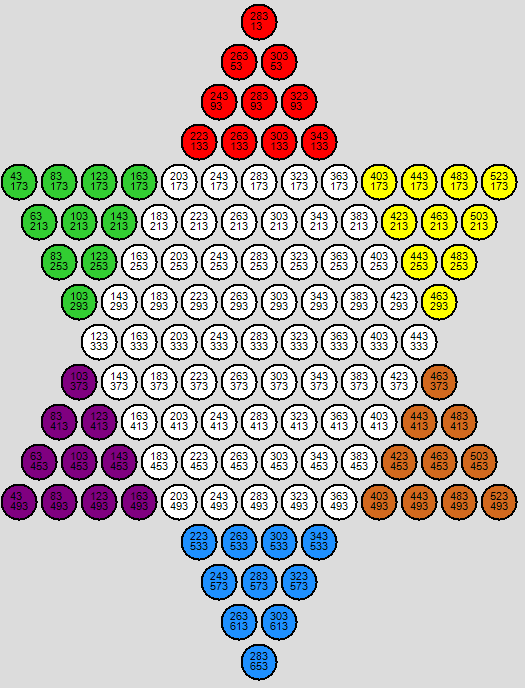
\includegraphics[width=0.7\textwidth]{Figures/SouradnicePoli.png}
	\caption{Souřadnice herních polí}
    \label{fig:SouradnicePoli}
\end{figure}

\section{Možné výsledky hry}
\label{sec:MozneVysledkyHry}
Po konci každého tahu je zkontrolováno, jestli se během daného tahu nepodařilo některému z hráčů přemístit všechny své kameny do daného cílového trojúhelníku. Hra může z pohledu lidského hráče skončit jedním ze čtyř výsledků:
\begin{description}
\item [výhra]  -- nastane v případě, že se lidskému hráči podaří přemístit všechny své kameny do cílového trojúhelníku jako prvnímu ze všech hráčů. Příklad lidským hráčem vyhrané hry můžeme vidět na obrázku číslo \ref{fig:Vyhra}.
\item [prohra]\index{prohra}  -- nastane v opačném případě než výhra, tedy tehdy, když se některému z počítačových hráčů povede přemístit všechny své kameny do daného cílového trojúhelníku dříve než lidskému hráči. Příklad lidským hráčem prohrané hry\index{prohra!hry} můžeme vidět na obrázku číslo \ref{fig:Prohra}.
\item [remíza]  -- relativně neobvyklý výsledek hry, nastává v případě, kdy se dvěma a více hráčům podaří přemístit všechny své kameny do daného cílového trojúhelníku během stejného tahu.~V~takovém případě hráč nevyhrál ani neprohrál, ale remizoval. Příklad takového výsledku hry můžeme vidět na obrázku číslo \ref{fig:Remiza}
\item [kontumace]\index{kontumace}  -- také se jedná o nepříliš častý výsledek hry, do hry je přidána jako ochrana proti taktice blokování. Nastává v případě, kdy hráč přemístil své kameny do všech volných polí cílového trojúhelníku a do zbývajících je nemůže přemístit výhradně z důvodu, že jsou obsazena hráčem, pro kterého je tento trojúhelník výchozím. Pro udělení kontumace\index{kontumace} je nutné splnění následující podmínky: součet kamenů patřících hráči, pro kterého je daný trojúhelník výchozím, nalézajících se ve třech polích nejbližších k cípu hvězdy a kamenů patřících hráči, pro kterého je daný trojúhelník cílovým, nalézajících se v celém trojúhelníku, musí být roven 10. V takovém případě už totiž hráč, který v trojúhelníku začínal, nemůže trojúhelník opustit bez toho, aniž by hráč, pro kterého je trojúhelník cílovým, neprovedl pro sebe nevýhodné tahy, kterými by mu uvolnil cestu k opuštění trojúhelníku. Grafické znázornění situací, při kterých nastává kontumace\index{kontumace}, je k dispozici na obrázku číslo \ref{fig:Kontumace}. Rozmístění kamenů ve třech polích nejbližších k cípu hvězdy je při kontumaci irelevantní, v potaz je bráno pouze splnění nebo nesplnění podmínky, jestli se kameny v těchto třech polích nacházejí. Stejně tak není brán ohled na polohu kamenů patřících hráči, pro kterého je trojúhelník cílový, nacházejících se mimo cílový trojúhelník, ohled je brán pouze na jeho kameny umístěné v cílovém trojúhelníku. Podmínky pro kontumaci jsou kontrolovány po každém tahu stejně jako podmínky pro vítězství. Pokud dojde ke kontumaci, je danému hráči přidělena kontumační výhra. Dá se ji tedy brát jako typ výhry, nicméně při ukončení hry je uvedeno, že hráč vyhrál kontumačně.
\end{description}
Po ukončení hry je uživateli ukázána zpráva o vítězícím hráči, uživatel se poté může vrátit do hlavního menu nebo může provést restartování hry, čímž vytvoří novou hru se stejnými parametry.

\begin{figure}
	\centering
	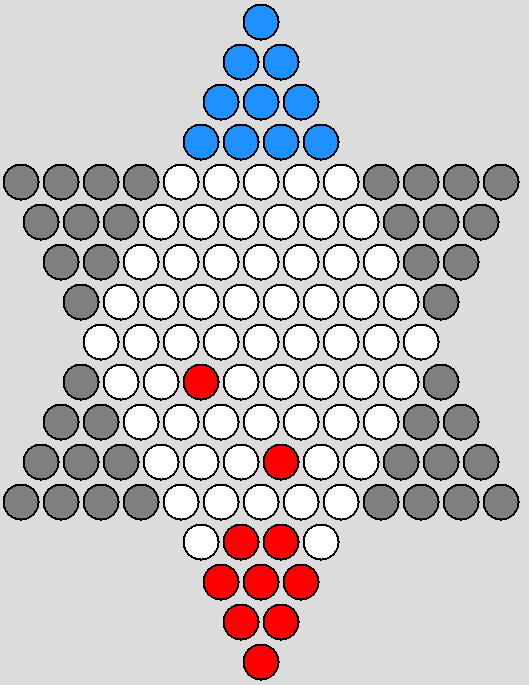
\includegraphics[width=0.4\textwidth]{Figures/Vyhra.png}
	\caption{Lidským hráčem vyhraná hra}
    \label{fig:Vyhra}
\end{figure}

\begin{figure}
	\centering
	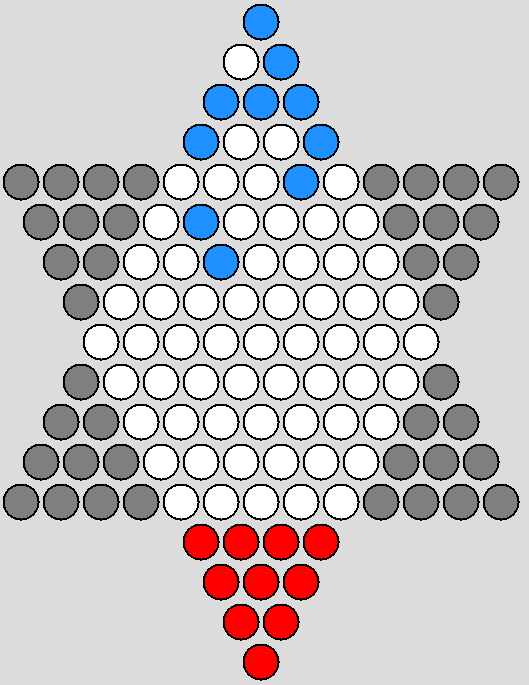
\includegraphics[width=0.4\textwidth]{Figures/Prohra.png}
	\caption{Lidským hráčem prohraná hra}
    \label{fig:Prohra}
\end{figure}

\begin{figure}
	\centering
	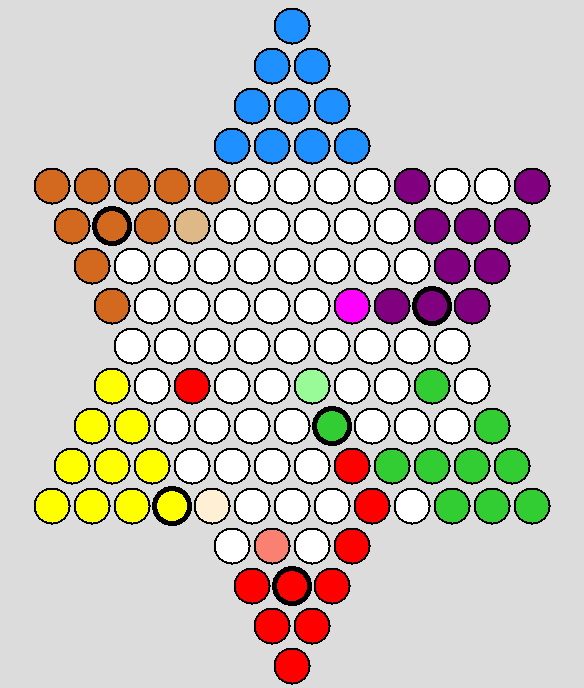
\includegraphics[width=0.4\textwidth]{Figures/Remiza.png}
	\caption[Příklad hry, ve které došlo k remíze]{Příklad hry, ve které došlo k remíze – během stejného tahu splnil podmínky výhry jak modrý (lidský) hráč, tak žlutý (počítačový) hráč}
    \label{fig:Remiza}
\end{figure}

\begin{figure}
	\centering
	\subfloat[Situace, kdy hráči v jeho výchozím trojúhelníku zbyl 1 kámen\label{fig:Kontumace1}]
	{
		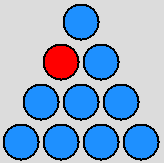
\includegraphics[width=0.35\textwidth]{Figures/Kontumace1.png}
	}
	\hspace{3em} % make more space
	\subfloat[Situace, kdy hráči v jeho výchozím trojúhelníku zbyly 2 kameny\label{fig:Kontumace2}]
	{
		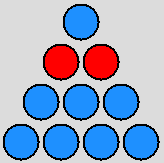
\includegraphics[width=0.35\textwidth]{Figures/Kontumace2.png}
	}
	\hspace{3em} % make more space
	\subfloat[Situace, kdy hráči v jeho výchozím trojúhelníku zbyly 3 kameny\label{fig:Kontumace3}]
	{
		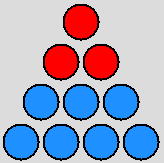
\includegraphics[width=0.35\textwidth]{Figures/Kontumace3.png}
	}
	\caption[Příklady situací, při kterých nastává kontumace]{Příklady situací, při kterých nastává kontumace\index{kontumace} (s ohledem na počet kamenů, který hráči zbyl v jeho výchozím trojúhelníku)}
	\label{fig:Kontumace}
\end{figure}
\endinput
\chapter{Počítačový hráč}
\section{Tahová logika}
Hráče na desce bychom si mohli rozdělit do dvou skupin v závislosti na nejrelevantnějších osách určujících jejich směr pohybu. U hráčů v nejnižším a nejvyšším cípu hvězdy (tedy v právě těch dvou cípech, které jsou využívány při hře dvou hráčů) je nejrelevantnější $y$-ová osa. Cílem těchto hráčů je totiž cíp mající polohu na $x$-ové ose shodnou s jejich výchozím cípem, a proto není důležitost polohy jejich tahů na $x$-ové ose příliš velká. U zbývajících čtyř hráčů toto ale neplatí vzhledem k~tomu, že jejich cílové cípy mají kromě odlišné polohy na $y$-ové ose odlišnou také polohu na $x$-ové ose. Pro tyto čtyři hráče je tedy velmi důležitá také poloha jejich tahů na $x$-ové ose. Z tohoto důvodu je implementace vykonávání pohybů pro obě tyto skupiny hráčů do značné míry odlišná. U popisu chování hráče proto vykonávaní pohybů pro obě tyto skupiny popisujeme odděleně. Názorná ukázka směrů, kterým hráči táhnou s ohledem na $x$-ové a $y$-ové souřadnice je na obrázku číslo \ref{fig:SmeryTahu}.

\begin{figure}
	\centering
	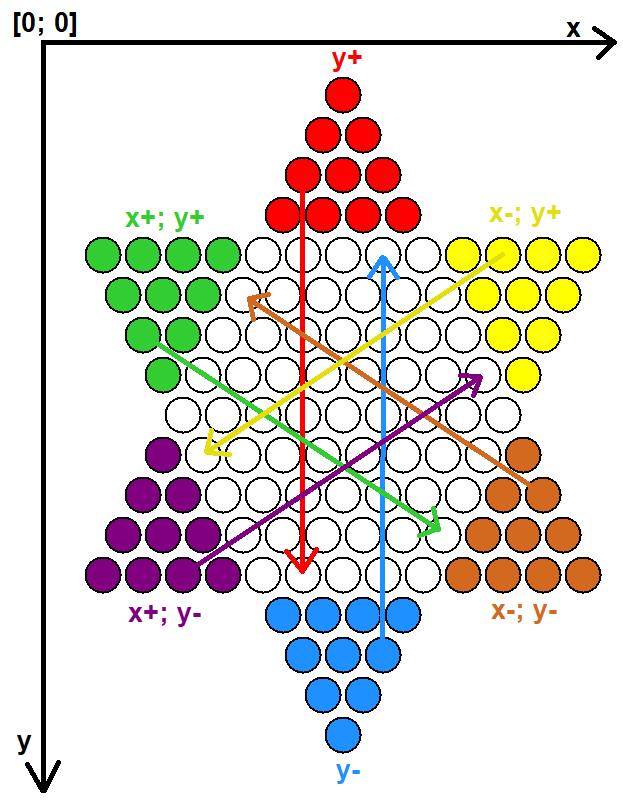
\includegraphics[width=0.7\textwidth]{Figures/SmeryTahu.png}
	\caption{Směry tahů hráčů s ohledem na $x$-ové a $y$-ové souřadnice}
    \label{fig:SmeryTahu}
\end{figure}

Existují ale i tahy, u kterých není okamžitá uražená vzdálenost nejdůležitějším parametrem. Asi nejtypičtějším příkladem takových tahů jsou prvotní tahy, tedy tahy vykonávané na začátku hry. V~ této práci je implementován prvotní tah Cross Caterpillar, jehož princip je vysvětlen v~podkapitole \ref{sec:Strategie}. Od klasických tahů se odlišují také tahy vykonávané na úplném konci hry. Na konci hry je totiž velmi vysoká pravděpodobnost, že kameny počítačového hráče jsou rozmístěny takovým způsobem, že je nutné provést tahy neodpovídající směrům uvedeným v obrázku číslo \ref{fig:SmeryTahu}. Příklad takové situace můžeme zhlédnout na obrázku číslo \ref{fig:SituaceNaKonciHry}. Odděleně implementované prvotní a koncové tahy ale nejsou vzhledem k existenci různých obtížností počítačových hráčů využívány vždy, využití těchto tahů je detailně rozebráno v následující podkapitole týkající se právě obtížností počítačových hráčů.

\begin{figure}
	\centering
	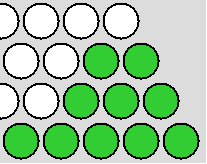
\includegraphics[width=0.4\textwidth]{Figures/SituaceNaKonciHry.png}
	\caption{Příklad situace na konci hry, kdy hráč musí provést tah v jiném než určeném směru}
    \label{fig:SituaceNaKonciHry}
\end{figure}

Dále je nutné při tazích počítačového hráče brát v potaz lidského hráče. Konkrétně je nutné zvažovat, jak provedení tahu počítačového hráče ovlivní lidského hráče. Je totiž dost pravděpodobné že během hry dojde k situaci, kdy počítačový hráč provede pro něj nejvýhodnější tah, jehož vykonání ale dá lidskému hráči možnost provést výhodnější tah, než jaký mohl provést před vykonáním tahu počítačového hráče. K zabránění vykonání takového tahu slouží metoda \lstinline$JeTahVyhodny$ ve třídě \lstinline$PohybPocitacovehoHrace$, která provede simulaci vykonání tahu počítačového hráče a zjistí, jestli může po jeho vykonání lidský hráč provést výhodnější tah než předtím. Metoda ale není využita vždy, stejně jako u předchozího odstavce i zde její využití závisí na obtížnosti počítačového hráče, využití je tedy popsáno v následující podkapitole.

Při tahu může nastat situace, kdy není možné provést žádný logický tah odpovídající směrům uvedeným na obrázku číslo \ref{fig:SmeryTahu}. Typicky může taková situace nastat při hře 6 hráčů ke konci hry, kdy už zbývá hráči do cílového trojúhelníku přesunout pouze několik kamenů, přičemž cesta je blokována kameny ostatních hráčů. V takovém případě je proveden náhodný tah, táhne se vždy ale pouze s některým z kamenů, který zatím není v cílovém trojúhelníku. 

\section{Úrovně obtížnosti}
\label{sec:UrovneObtiznosti}
Při vytváření her, ve kterých lidský hráč bojuje proti počítačovým hráčům, je jedním z hlavních cílů vytvořit lidskému hráči rovnocenného, tedy co nejsilnějšího protivníka. Je ovšem také nutné brát v~potaz rozdílné dovednostní úrovně lidských hráčů -– začátečník jistě nebude ve hře tak dobrý jako zkušený hráč. Z tohoto důvodu jsou v této hře implementovány tři různé obtížnosti počítačových nepřátel. Před začátkem hry pak lidský hráč nastaví obtížnost jeho počítačových nepřátel.

Nejprve rozebereme počítačového hráče s nejnižší úrovní obtížnosti, dále bude označován jako \emph{lehký}. U hráčů v nejvýše a nejníže položeném trojúhelníku je během každého tahu proveden pohyb, který je neposune směrem opačným vzhledem k jejich cíli na $y$-ové ose. Jinak řečeno, kámen musí být během tahu posunut blíže k cíli, nebo musí zůstat stejně daleko (týká se pouze $y$-ové osy, na $x$-ovou osu není brán zřetel). U zbývajících čtyř hráčů je pak nutné, aby byl tah veden~v~obou směrech znázorněných na obrázku číslo \ref{fig:SmeryTahu}. Například kámen zeleného hráče musí být vždy přemístěn do pole, které má vyšší $x$-ovou i $y$-ovou souřadnici než samotný kámen. Není vybírán nejvýhodnější tah, z možných tahů splňujících zmíněnou podmínku je vždy náhodně vybrán jeden z nich.

Další je počítačový hráč s vyšší úrovní obtížnosti, ten bude dále označován jako \emph{střední}. Ten funguje na podobném principu jako lehký hráč, z proveditelných tahů je také vždy vybrán jeden z~nich, liší se v podmínkách proveditelnosti tahů. U hráčů v nejvýše a nejníže položeném trojúhelníku je nutné, aby byl kámen během tahu posunut blíže k cíli na $y$-ové ose. Proti lehkému hráči se liší v tom, že kámen nemůže během tahu zůstat na $y$-ové ose stejně daleko k cíli. U zbývajících čtyř hráčů je pak nutné, aby byl tah veden v alespoň jednom ze směrů uvedeném na obrázku číslo \ref{fig:SmeryTahu}. Kámen zeleného hráče musí tedy být přemístěn do pole, které má vyšší buď $x$-ovou, nebo $y$-ovou souřadnici. Mohlo by se zdát, že je kvůli tomuto rozdílu střední hráč slabší než lehký hráč, ale není tomu tak. Lehký hráč sice projde herní deskou rychleji, znatelný rozdíl ale nastane v závěrečné fázi hry -– zatímco střední hráč své kameny rozloží rovnoměrně do celého cílového trojúhelníku, lehký hráč nejdříve obsadí okraje sousedící s nejvýše nebo nejníže položeným trojúhelníkem (v závislosti na poloze cílového trojúhelníku). Kvůli tomu lehký hráč potřebuje k dokončení hry mnohem větší počet tahů než střední hráč.

Posledním nezmíněným hráčem je počítačový hráč s nejvyšší úrovní obtížnosti, dále bude označován jako \emph{těžký}. Tento hráč se od lehkého i středního hráče velmi zásadně liší. Během každého tahu je vždy proveden nejvýhodnější možný pohyb, jeho tahy tedy nikdy nejsou náhodné. U hráčů v nejvýše a nejníže položeném trojúhelníku je vždy proveden tah, který hráče posune co nejblíže k cíli na $y$-ové ose. V potaz je zde ale brána i $x$-ová osa -– z tahů nejvýhodnějších podle $y$-ové osy je proveden ten z nich, který hráče posune nejblíže k středu mapy. U zbývajících hráčů je pak proveden tah, který je dostane nejdál ve směru uvedeném v obrázku číslo \ref{fig:SmeryTahu}. U hráčů v nejvýše a nejníže položeném trojúhelníku je prováděn počáteční tah Cross Caterpillar (u zbývajících hráčů prováděn není vzhledem k tomu, že jeho provedení u nich ve výsledku zvýší počet tahů potřebný pro vítězství). U všech hráčů s touto obtížností jsou také ošetřeny koncové tahy, což výrazně sníží počet tahů potřebných k vítězství. Je zde taktéž kladen důraz na možné budoucí tahy lidského hráče, pro tyto účely je využívána metoda \lstinline$JeTahVyhodny$ popsaná v předchozí podkapitole.

Výpis všech relevantních dovedností a schopností jednotlivých počítačových hráčů podle jejich obtížnosti se nachází v tabulce číslo \ref{tab:ObtiznostiPocitacovychHracu}.

\begin{table}
	\centering
	\caption{Dovednosti a vlastnosti počítačových hráčů podle obtížnosti}
	\label{tab:ObtiznostiPocitacovychHracu}
	\begin{tabular}{cccc}
		\toprule
		Vlastnost & \multicolumn{1}{c}{Lehký} & \multicolumn{1}{c}{Střední} & \multicolumn{1}{c}{Těžký}\\
		\midrule
		Zajištěna výhra v rozumném počtu tahů & \faTimes & \faCheck & \faCheck\\
		Náhodné pohyby & \faCheck & \faCheck & \faTimes\\
		Vykonání nejvýhodnějšího tahu & \faTimes & \faTimes & \faCheck\\
		Brán ohled na tahy lidského hráče & \faTimes & \faTimes & \faCheck\\
		Počáteční pohyby & \faTimes & \faTimes & \faCheck*\\
		Koncové pohyby & \faTimes & \faTimes & \faCheck\\
		\bottomrule
	\end{tabular}
	\begin{tablenotes}
      \small
      \item *U hráčů v nejvýše a nejníže položeném trojúhelníku
    \end{tablenotes}
\end{table}

\section{Simulátor}
Pro praktickou ukázku síly jednotlivých počítačových hráčů podle jejich obtížností je v aplikaci implementován simulátor. Ten je spravován samotným uživatelem, který si může navolit počet hráčů a obtížnosti jednotlivých hráčů. Tito hráči budou poté hrát proti sobě bez dalšího zásahu uživatele. 

Tyto simulace je možné provádět dvěma způsoby. Uživatel může buďto nechat provést simulaci o~daných parametrech pouze jednou, nebo může nechat provést větší množství simulací o daných parametrech po sobě. Dá se tedy říct, že druhý způsob slouží spíše k statistickým účelům než k~sledování průběhu konkrétní hry. Z toho důvodu je uživateli promítnut průběh hry a výsledek pouze během provádění jediné simulace. U obou způsobů provádění simulací je nicméně výsledek zaznamenán do souboru \textsf{Statistiky.txt}, který se nachází v kořenovém adresáři aplikace. Do záznamu je uložen počet hráčů, počet tahů, obtížnost jednotlivých hráčů a výsledek simulace. Uživatel může všechny uložené statistiky nalézt i v samotné aplikaci, jsou dostupné v hlavním menu po výběru možnosti \textsf{Statistiky}.

V této práci je simulátor využit pro ukázku dovedností počítačových hráčů podle jejich obtížností v kapitole \ref{sec:HryMeziPocitacovymiHraci}.
\endinput
\chapter{Implementace}
\section{Využité technologie}
Aplikace byla vytvořena za použití nástroje Microsoft Visual Studio 2019, což je populární vývojové prostředí (IDE) vyvíjené firmou Microsoft. Toto prostředí je, co se týče programování aplikací pro operační systém Windows vyvíjený stejnojmennou firmou, standardem. Také u naší aplikace se proto počítá s využitím zmíněného operačního systému k jejímu provozu. Využíván je také .NET Framework \cite{net-framework}, což je platforma sloužící vývojářům k vytváření a spouštění aplikací. Tato platforma má velké množství verzí, u této aplikace počítáme s využitím verze .NET Framework 4.7.2. Naší aplikaci bychom mohli kategorizovat jako aplikaci s grafickým uživatelským rozhraním (GUI), což je pojem známý spíše pod svým anglickým jménem „Windows Application“. Pro implementaci uživatelského rozhraní je v případě této aplikace využita knihovna tříd Windows Forms \cite{winforms}, která je také součástí .NET Frameworku. K naprogramování celé aplikace byl využit programovací jazyk C\#, což je objektově orientovaný jazyk vyvíjený taktéž firmou Microsoft.

\section{Objektová analýza}
Třídy obsažené v aplikaci bychom mohli podle jejich funkce rozdělit na dvě skupiny.
\begin{itemize}
	\item Ovládání hry
		\begin{itemize}
		\item \lstinline$Hra$
		\item \lstinline$PohybPocitacovehoHrace$
		\item \lstinline$VypocetMoznychTahu$
	\end{itemize}
	\item Herní entity
		\begin{itemize}
		\item \lstinline$LidskyHrac$
		\item \lstinline$MoznyTahLidskehoHrace$
		\item \lstinline$MoznyTahLPocitacovehoHrace$
		\item \lstinline$PocitacovyHrac$
		\item \lstinline$Pole$
		\item \lstinline$VychoziPolePocitacovehoHrace$
		\item \lstinline$ZvyrazneniPoleLidskehoHrace$
		\item \lstinline$ZvyrazneniPolePocitacovehoHrace$
	\end{itemize}
\end{itemize}

U některých entit bychom si mohli všimnout rozdělení na entity lidského a počítačového hráče. Tyto entity (tedy možný tah, pole hráče a zvýraznění pole) mají vlastní objekty a využívají vlastní kolekce, a to i přes to, že mají stejné nebo velmi podobné parametry i metody. Jistě by tedy šlo použít jediný objekt a jedinou kolekci pro všechny hráče a funkčnost aplikace by zůstala beze změny. Důvod pro jejich rozdělení je jednoduchý -– s entitami lidského a počítačových hráčů pracujeme vždy odděleně, takže rozdělení jejich objektů ve výsledku výrazně usnadní práci s těmito objekty. Pokud bychom objekty neoddělili, museli bychom při každé iteraci kolekce některé ze skupin objektů specifikovat, kterého hráče se daná iterace týká. Takový postup by vzhledem k vysokému počtu cyklů nacházejících se v programu značně ztížil jakoukoli manipulaci s danými objekty, a navíc by zde byl prostor k neúmyslnému vytváření obtížně vysledovatelných chyb.

Pro upřesnění je na obrázku \ref{fig:TridniDiagram} k dispozici třídní diagram celé aplikace. U tříd z kategorie \emph{Herní entity} bylo vzhledem k menšímu počtu parametrů a metod možné do diagramu zaznamenat vše, u tříd z kategorie \emph{Ovládání hry} jsou ale uvedeny jen některé (zpravidla nejdůležitější) parametry a metody. Pro úsporu místa jsou také v diagramu používány zkratky, například u třídy \lstinline$PohybPocitacovehoHrace$ namísto „PocitacovyHrac“ zapisujeme \enquote{PHrac}.

\begin{figure}
	\centering
	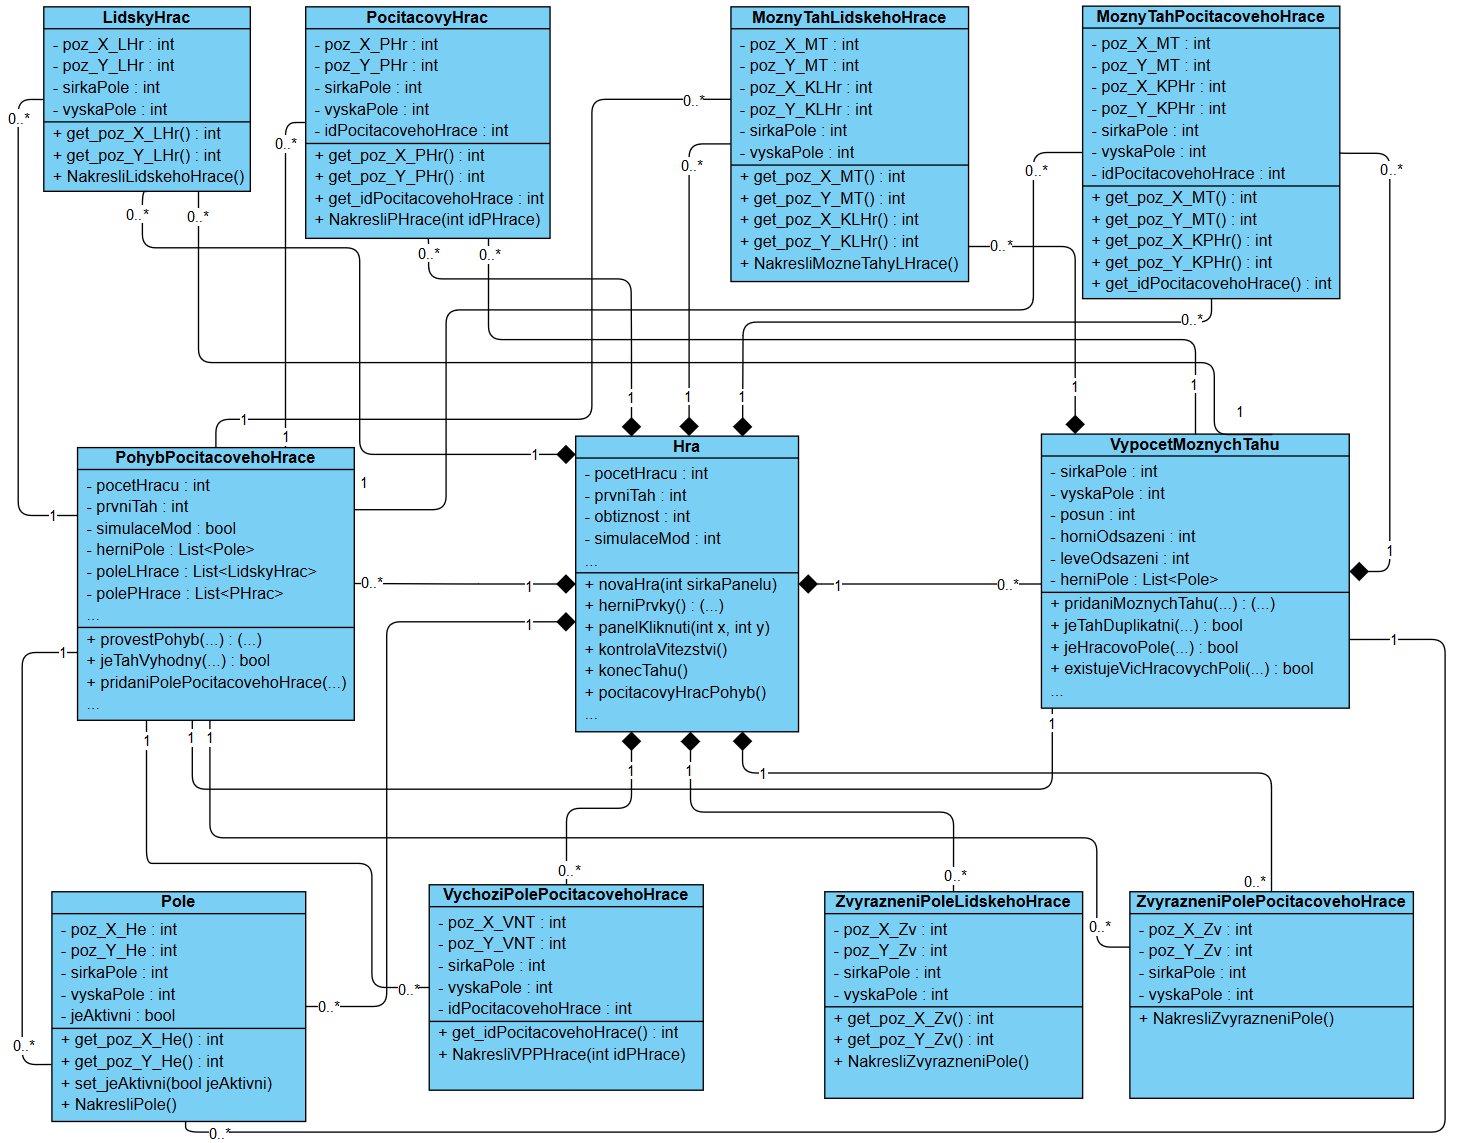
\includegraphics[width=1\textwidth]{Figures/TridniDiagram.png}
	\caption{Třídní diagram aplikace Čínská dáma}
    \label{fig:TridniDiagram}
\end{figure}

\section{Vytvoření a provoz hry}
\label{sec:VytvoreniAProvozHry}
Hra je vytvořena zavoláním metody \lstinline$NovaHra$ třídy \lstinline$Hra$. Toto volání probíhá v konstruktoru třídy \lstinline$HraForm$, což je třída, prostřednictvím které hráč ovládá hru a sleduje její aktuální stav. V konstruktoru je taktéž vytvářena instance třídy \lstinline$Hra$, přičemž jsou do třídy Hra předány parametry, které nastavuje uživatel. Předáván je tímto způsobem počet hráčů, dále informace o tom, jestli se jedná o simulaci a obtížnost počítačových hráčů. Mimo to si uživatel může také zvolit, jestli bude první na tahu on, nebo počítačový hráč (nabízí se i možnost vybrat začínajícího hráče náhodně, což by odpovídalo hodu mincí, který může být využíván k určení začínajícího hráče u her na fyzické herní desce). 

V metodě \lstinline$NovaHra$ nejprve dochází k vytvoření herní desky (tento proces je blíže vysvětlen v~podkapitole \ref{sec:HerniPole}). Po vytvoření herního pole jsou vytvořena pole lidského a počítačových hráčů. Každý hráč má unikátní ID, které je využíváno mimo jiné při kontrole vítězství u jednotlivých hráčů. Přidělování ID funguje na stejném principu jako přidělování barev, přidělováno je vždy na základě výchozího trojúhelníku hráče, nezávisle na počtu hráčů. Ukázku systému přidělování ID na základě výchozího trojúhelníku můžeme vidět na obrázku číslo \ref{fig:IDPocitacovychHracu}. Na zmíněném obrázku je k~modrému hráči přiděleno ID 0. Nejedná se o lidského hráče (který má přidělené ID 1), jedná se o~modrého počítačového hráče, který je ale využíván pouze při simulacích.

\begin{figure}
	\centering
	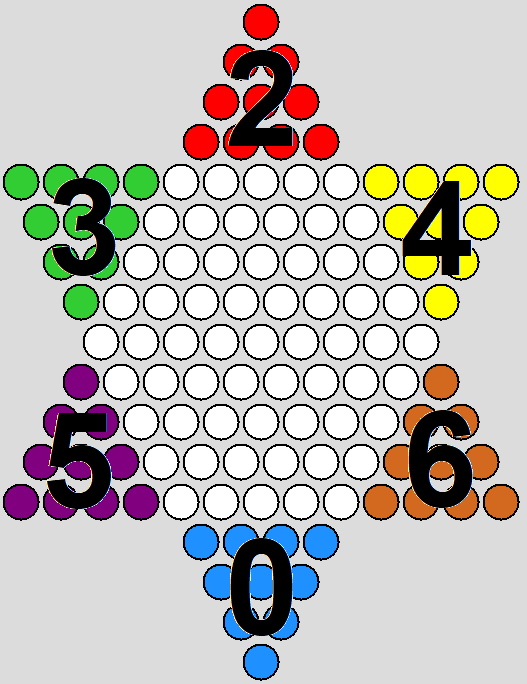
\includegraphics[width=0.4\textwidth]{Figures/IDPocitacovychHracu.png}
	\caption{Počítačoví hráči podle jejich ID}
    \label{fig:IDPocitacovychHracu}
\end{figure}

Hráči jsou vytvářeni na základě splnění podmínek. Jednak musí být pro jejich vytvoření nastaven odpovídající počet hráčů. Dále jsou v cyklu procházena všechna herní pole a probíhá kontrola, jestli se má na daném poli nacházet daný počítačový hráč. U hráčů v nejvýše a nejníže položeném trojúhelníku je tato kontrola velmi jednoduchá -– záleží pouze na $y$-ové poloze daného pole.~U~zbývajících čtyř hráčů je ale tato kontrola o poznání složitější -– záleží jak na $y$-ové poloze, tak na $x$-ové.

Pro umožnění znovupoužitelnosti a snadnější čitelnost kódu jsou tyto podmínky uloženy v metodě \lstinline$JePoleVHornimLevemRohu$, do které jsou vyslány souřadnice daného pole a je vrácena informace o tom, jestli se pole v daném trojúhelníku nachází nebo ne. Metody fungující na stejném principu jsou samozřejmě vytvořeny pro každý trojúhelník obsažený ve hvězdě.

Po vytvoření všech zmíněných polí je hra připravená. Hru ovládá uživatel (lidský hráč) kliknutím na některé ze svých herních polí a následně kliknutím na některý z možných tahů (průběh zpracování možných tahů je vysvětlen v následující podkapitole). Po dokončení hráčova tahu jsou na tahu počítačoví hráči. Je zavolána metoda \lstinline$KonecTahu$, ve které proběhne zavolání metody \lstinline$ProvestPohyb$ ve třídě \lstinline$PohybPocitacovehoHrace$, do které je posláno aktuální rozložení herní desky a jejímž návratovým typem je rozložení herní desky s novými pozicemi počítačových hráčů. Počítačoví hráči jsou v této metodě procházeni v cyklu a v každé iteraci je určen tah vždy jednoho počítačového hráče. 

\section{Vytvoření možných tahů}
\label{sec:VytvoreniMoznychTahu}
Jak už bylo zmíněno v podkapitole \ref{sec:MozneTahy}, aplikace podporuje tahy na sousední pole a skoky, pohyby je možné provádět v šesti směrech. V této podkapitole je prezentována implementace tahů na sousední pole a také skoku v jednom z šesti směrů. Postup vytvoření možných tahů a výběru některého z~nich by se dal shrnout v následujících bodech:
\begin{enumerate}
	\item Lidský hráč klikne na jeden ze svých kamenů
\item\label{moznyTahPostup} Aplikace zvýrazní daný kámen a světle modře vyznačí všechna pole, na která se hráč může přesunout
\item Lidský hráč si kliknutím vybere jedno z nabízených polí
	\item Aplikace po výběru pole vyhodnotí další postup
	\begin{enumerate}
		\item hráč si vybral sousední pole, jeho tah je ukončen
		\item hráč provedl skok, aplikace provede stejný postup jako v bodě \ref{moznyTahPostup}, hráč může provést libovolné množství skoků, tah poté ukončí kliknutím na zvýrazněné pole nebo na tlačítko v kontrolním panelu
	\end{enumerate}
	\item Tah lidského hráče skončil, aplikace odstraní kámen na původní poloze a vytvoří kámen na právě vybrané poloze, na tahu jsou nyní počítačoví hráči
\end{enumerate}

Když hráč klikne na jeden ze svých kamenů, jsou v metodě \lstinline$PanelKliknuti$ třídy \lstinline$Hra$ v cyklu procházena všechna herní pole, přičemž v každé iteraci je kontrolováno, jestli pole splňuje podmínky pro to, aby bylo přidáno jako možný tah. Na začátku každé iterace je ještě zkontrolováno, jestli se pole nenachází v jiném než výchozím nebo cílovém trojúhelníku daného hráče, do těchto polí totiž hráč nemá přístup. Nejprve budou prezentovány podmínky pro vytvoření možného tahu na sousedních polích. Podmínky i s vysvětlivkami jsou k dispozici ve výpisu číslo \ref{src:moznyTahSousedniPole}.

\begin{lstlisting}[label=src:moznyTahSousedniPole,caption={Podmínky pro vytvoření možného tahu - sousední pole}]
Math.Abs(poz_Y_KHr - poz_Y_He) <= posun /*vzdálenost kliknutého hráčova pole a právě procházeného herního pole není větší než dané odsazení mezi herními poli (na y-ové ose)*/ &&
Math.Abs(poz_X_KHr - poz_X_He) <= posun /*vzdálenost kliknutého hráčova pole a právě procházeného herního pole není větší než dané odsazení mezi herními poli (na x-ové ose)*/ &&
!JeTahDuplikatni(poz_X_He, poz_Y_He, poz_X_KHr, poz_Y_KHr, idHrace, mozneTahyLidskehoHrace, mozneTahyPocitacovehoHrace) /*tah není duplikátní (na daném poli se již nenachází možný tah daného hráče)*/ &&
!JeHracovoPole(poz_X_He, poz_Y_He, poleLidskehoHrace, polePocitacovehoHrace) /*na daném poli není žádné hráčovo nebo nepřítelovo pole*/ &&
!hracSePohlSkokem /*hráč neprovedl ve svém tahu skok -- tahy na sousední pole a skoky nelze během jednoho tahu kombinovat*/
\end{lstlisting}

Následují možné tahy vykonávané prostřednictvím skoků. Ty už jsou jak na porozumění, tak na implementaci složitější než tahy na sousední pole. Při provedení skoku je ve třídě Hra do proměnných \lstinline$delkaSkokuX$ a \lstinline$delkaSkokuY$ uložena délka skoku na $x$-ové, resp. $y$-ové ose. Jedná se o vzdálenost pole, na kterém se nacházel přesouvaný kámen a pole, na které byl kámen přemístěn na daných osách. Při skoku je také nastavena proměnná \lstinline$hracProvedlSkok$ na \lstinline$true$, což je využito k zamezení přidání sousedních polí jako možných tahů po provedení skoku. V metodě \lstinline$PridaniMoznychTahu$ už v cyklu neprocházíme pouze herní pole (jako u tahů na sousední pole), ale také pole lidského a počítačových hráčů, protože právě tato pole jsou během skoků přeskakována. Pro příklad budou prezentovány pouze skoky v nevodorovném směru, tedy skoky, u kterých je délka skoku na $y$-ové ose vyšší než 0. Nevodorovné a vodorovné skoky lze kombinovat, jejich princip je ale až na absenci podmínek týkajících se $y$-ové osy u prvního vodorovného skoku stejný. Podmínky pro vytvoření možného tahu u pole, na které by se hráč přesunul skokem, nalezneme ve výpisu \ref{src:moznyTahSkokyPrvni}.

\begin{lstlisting}[label=src:moznyTahSkokyPrvni,caption={Podmínky pro vytvoření možného tahu - skoky (první skok)}]
(poz_X_Hr - poz_X_KHr == poz_X_He - poz_X_Hr) /*vzdálenost právě procházeného hráčova pole a kliknutého hráčova pole je stejná jako vzdálenost právě procházeného herního pole a právě procházeného hráčova pole (na x-ové ose)*/ &&
(poz_Y_Hr - poz_Y_KHr == poz_Y_He - poz_Y_Hr) /*vzdálenost právě procházeného hráčova pole a kliknutého hráčova pole je stejná jako vzdálenost právě procházeného herního pole a právě procházeného hráčova pole (na y-ové ose)*/ &&
(Math.Abs(poz_Y_KHr - poz_Y_He) == 2 * Math.Abs(poz_X_KHr - poz_X_He)) /*vzdálenost kliknutého hráčova pole a právě procházeného herního pole na y-ové ose je dvakrát větší než vzdálenost kliknutého hráčova pole a právě procházeného herního pole na x-ové ose*/ &&
!JeTahDuplikatni(poz_X_He, poz_Y_He, poz_X_KHr, poz_Y_KHr, idHrace, mozneTahyLidskehoHrace, mozneTahyPocitacovehoHrace) &&
!JeHracovoPole(poz_X_He, poz_Y_He, poleLidskehoHrace, polePocitacovehoHrace) &&
!ExistujeVicHracovychPoli(poz_X_KHr, poz_Y_KHr, poz_X_He, poz_Y_He, poleLidskehoHrace, polePocitacovehoHrace) /*mezi kliknutým hráčovým polem a právě procházeným herním polem se nachází právě jedno hráčovo pole*/ &&
!hracSePohlSkokem 
\end{lstlisting}

V předchozím výpisu probíhá v cyklu herních polí vnořený cyklus s poli lidského hráče. Po provedení tohoto cyklu následuje vzhledem k oddělení polí lidského a počítačových hráčů vnořený cyklus s poli počítačových hráčů, u kterého jsou pro přidání množného tahu stejné podmínky jako u cyklu s poli lidského hráče. 

Předchozí výpis týkající se skoků platí pouze pro skok provedený na začátku tahu. U skoku na začátku tahu se při jeho vyhodnocování nebere ohled na délku skoku, ta je pouze zaznamenávaná. U všech zbývajících skoků v rámci tahu nicméně musíme brát na délku skoku ohled, všechny skoky provedené v rámci jednoho tahu musí mít stejnou velikost, tedy délka skoku u prvního skoku v tahu určuje rovněž délku všech ostatních skoků v tahu. 

Po výběru možného tahu je v metodě \lstinline$PanelKliknuti$ zkontrolováno, jestli se hráč posunul na sousední pole, nebo jestli provedl skok. V případě, že provedl skok, je pro hráčův přesunutý kámen na jeho nové poloze opět proveden výpočet možných tahů, tentokrát už ovšem se zaznamenanou délkou skoku, což umožní splnění podmínky, aby byla délka skoku u všech skoků v tahu totožná. Tento postup umožní řetězení skoků, tedy provedení více skoků v jednom tahu. Přidání možných tahů probíhá opět v metodě \lstinline$PridaniMoznychTahu$, příklad prezentující podmínky pro přidání možných tahů pro druhý a další skok (opět pouze v nevodorovném směru) nalezneme ve výpisu číslo \ref{src:moznyTahSkokyDalsi}.

\begin{lstlisting}[label=src:moznyTahSkokyDalsi,caption={Podmínky pro vytvoření možného tahu - skoky (druhý a další skok)}]
(Math.Abs(poz_X_KHr - poz_X_He) == delkaSkokuX) /*vzdálenost mezi kliknutým hráčovým polem a právě procházeným herním polem je stejná jako délka skoku (na x-ové ose)*/&&
(Math.Abs(poz_X_He - poz_X_Hr) == delkaSkokuX / 2) /*vzdálenost mezi právě procházeným herním polem a právě procházeným hráčovým polem je dvakrát menší než délka skoku na x-ové ose */&&
(Math.Abs(poz_X_He - poz_X_KHr) == delkaSkokuY / 2) /*vzdálenost mezi právě procházeným herním polem a kliknutým hráčovým polem na x-ové ose je dvakrát menší než délka skoku na y-ové ose*/&&
(Math.Abs(poz_Y_KHr - poz_Y_He) == delkaSkokuY) /*vzdálenost mezi kliknutým hráčovým polem a právě procházeným herním polem je stejná jako délka skoku (na y-ové ose)*/ &&
(Math.Abs(poz_Y_KHr - poz_Y_Hr) == delkaSkokuY / 2) /*vzdálenost mezi kliknutým hráčovým polem a právě procházeným hráčovým polem je dvakrát menší než délka skoku (na x-ové ose)*/ &&
(poz_Y_Hr - poz_Y_KHr == poz_Y_He - poz_Y_Hr) /*vzdálenost mezi právě procházeným hráčovým polem a kliknutým hráčovým polem je stejná jako vzdálenost mezi právě procházeným herním polem a právě procházeným hráčovým polem (na y-ové ose)*/ &&
(poz_X_Hr - poz_X_KHr == poz_X_He - poz_X_Hr) /*vzdálenost mezi právě procházeným hráčovým polem a kliknutým hráčovým polem je stejná jako vzdálenost mezi právě procházeným herním polem a právě procházeným hráčovým polem (na x-ové ose)*/ &&
!JeTahDuplikatni(poz_X_He, poz_Y_He, poz_X_KHr, poz_Y_KHr, idHrace, mozneTahyLidskehoHrace, mozneTahyPocitacovehoHrace) &&
!JeHracovoPole(poz_X_He, poz_Y_He, poleLidskehoHrace, polePocitacovehoHrace) &&
!ExistujeVicHracovychPoli(poz_X_KHr, poz_Y_KHr, poz_X_He, poz_Y_He, poleLidskehoHrace, polePocitacovehoHrace)
\end{lstlisting}

Stejně jako u výpisu týkajícího se prvního skoku v daném tahu, popisován je zde vnořený cyklus s poli lidského hráče, po jeho vykonání následuje další vnořený cyklus, ve kterém jsou procházena pole počítačových hráčů.

\section{Vyhodnocení hry} 
Hra může z pohledu lidského hráče skončit čtyřmi způsoby (viz podkapitola \ref{sec:MozneVysledkyHry}). Po dokončení tahu všech hráčů je tedy nutné zkontrolovat, jestli některý z hráčů nesplnil svým posledním tahem podmínky k vítězství (všechny jeho kameny se nacházejí v cílovém trojúhelníku). Tato kontrola probíhá v metodě \lstinline$KontrolaVitezstvi$ třídy \lstinline$Hra$, jsou v ní postupně zkontrolovány kameny všech hráčů, a~ pokud některý z nich splnil podmínky vítězství, je lidský hráč uvědomen o ukončení hry a~o~jejím výsledku.

U této metody je potřeba zvážit několik okolností. Kromě výhry a prohry je možná také remíza, takže není možné v reakci na zjištění, že některý z hráčů splnil podmínky k vítězství ihned ukončit hru. Je nutné nejprve nechat táhnout všechny hráče a až poté zjišťovat, jestli některý z nich právě nevyhrál hru. Dále je nutné brát na zřetel, který hráč byl první na tahu – na začátku hry si lidský hráč může zvolit, jestli bude první na tahu on, nebo počítačoví hráči. Je tedy nutné postupovat tak, že pokud byl první na tahu lidský hráč, kontrolujeme vítězství hráčů vždy po tahu počítačových hráčů, a naopak pokud byl první na tahu počítačový hráč, kontrolujeme vítězství vždy po tahu lidského hráče. Pokud bychom nebrali začínajícího hráče na zřetel, tak bychom mohli některého hráče v případě velmi těsného výsledku znevýhodnit.

U kontroly vítězství je možné k určení vítězství hráče využít funkce implementované už při vytváření hráčových polí -– výchozí trojúhelník hráče je totiž pro hráče který je mu protilehlý cílovým trojúhelníkem. Kromě výhry, prohry, a remízy může ještě nastat kontumace (o přesných podmínkách kontumace hry pojednává taktéž podkapitola \ref{sec:MozneVysledkyHry}). Kontumace je kontrolována v metodě \lstinline$KontrolaKontumace$ třídy \lstinline$Hra$, v této třídě jsou implementovány metody fungující na stejném principu jako metoda \lstinline$JePoleVHornimLevemRohu$ třídy \lstinline$Hra$, z této metody jsou volány funkce kontrolující počet kamenů v jednotlivých trojúhelnících hvězdy, které ale v tomto případě střídavě zvažují, jestli má být kontrolován celý trojúhelník nebo pouze tři pole nejblíž k cípu trojúhelníku, pouze tato pole jsou totiž v případě kontumace zvažována u kamenů hráče, pro kterého je trojúhelník výchozím.
\endinput
\chapter{Uživatelské rozhraní}
\section{Herní okno}
Bezpochyby nejdůležitějším oknem obsaženým v aplikaci je okno sloužící k vyobrazení průběhu samotné hry. V aplikaci jej najdeme pod názvem \lstinline$HraForm$, v této práci pak jako obrázek číslo \ref{fig:HerniOkno}.

\begin{figure}
	\centering
	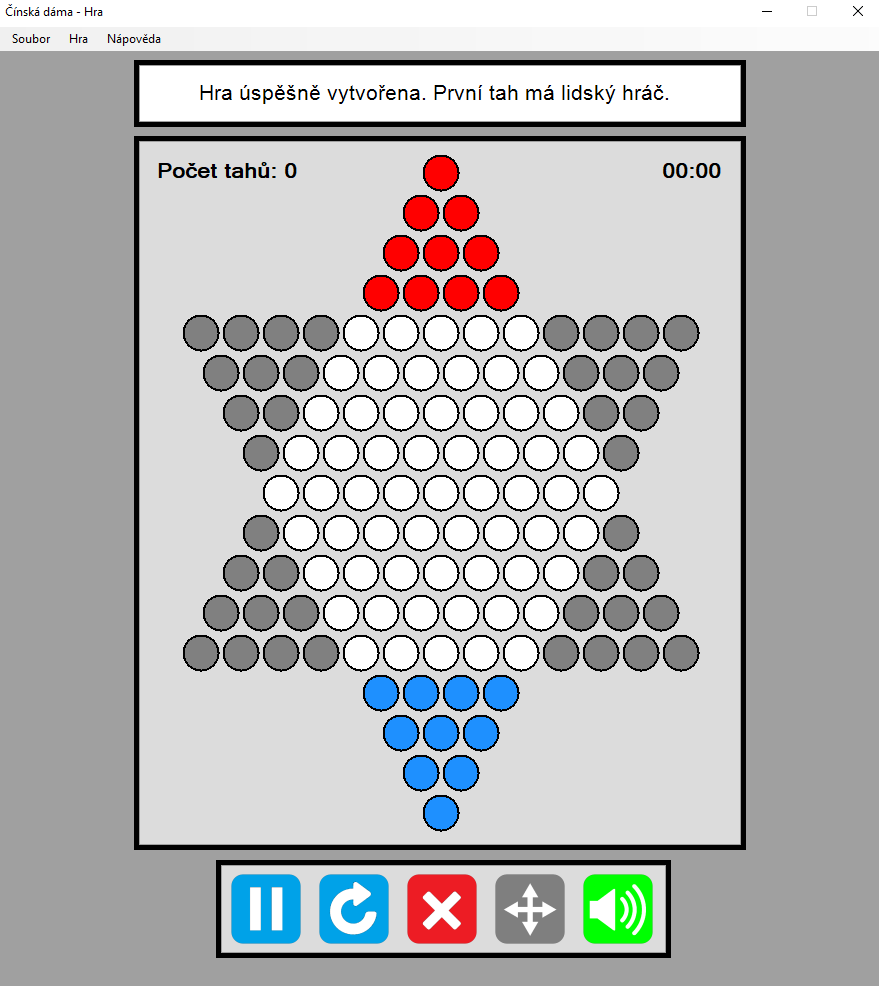
\includegraphics[width=0.7\textwidth]{Figures/HerniOkno.png}
	\caption{Herní okno aplikace}
    \label{fig:HerniOkno}
\end{figure}

Herní okno je tvořeno třemi částmi. Odshora první částí je informační panel, který slouží jako dodatečný prostředek k informování uživatele o průběhu hry. Na obrázku \ref{fig:HerniOkno} obsaženém v této práci informuje uživatele o úspěšném vytvoření hry a prvním hráči na tahu, kromě toho informační panel vypisuje také informace o výsledku her nebo simulací a také během provádění pohybů počítačových hráčů informuje uživatele o tom, pro kterého počítačového hráče je právě vypočítáván tah. Zejména u her s větším množstvím počítačových hráčů vyšších obtížností totiž trvá provedení tahu pro všechny počítačové hráče i několik sekund, a uživatel by mohl nabýt dojmu, že aplikace přestala reagovat. Informační panel také informuje hráče o případném pozastavení hry.

Pod informačním panelem se pak nachází okno zobrazující průběh samotné hry. V aplikaci nese název \lstinline$herniPanel$, a obsahuje dvě naprosto nezbytné události -– událost \lstinline$Paint$, která umožňuje vykreslování jednotlivých objektů, a událost \lstinline$MouseClick$, která reaguje na uživatelova kliknutí myší, což umožní uživateli přesouvání svých kamenů po herní desce. Podrobněji je komunikace mezi herním oknem a hrou popsána v následující podkapitole.

Pro implementaci okna zobrazujícího průběh hry byla nejprve využita třída \lstinline$Panel$. Ta je u~méně rozsáhlých aplikací adekvátním řešením, nicméně u této aplikace se využívá poměrně vysoké množství objektů, a pravděpodobně z tohoto důvodu bylo při hře patrné nepříjemné blikání celé herní desky. Proto je namísto třídy \lstinline$Panel$ využita třída \lstinline$DoubleBufferedPanel$ \cite{doublebuffered}, která z třídy panel dědí. Při využití vlastnosti \lstinline$DoubleBuffered$ překresluje prvek svou plochu pomocí sekundární vyrovnávací paměti, což ve výsledku zabrání blikání.

Mimo to je v tomto okně zobrazena informace o počtu tahů a o uběhlém čase. Vlevo nahoře je vyznačen počet tahů, který je v tomto kontextu chápán jako počet kol, ve kterých všichni hráči táhli, nikoli jako součet počtů tahů všech hráčů. Vpravo nahoře se pak nalézá časomíra, která v~minutách a sekundách měří čas uplynulý od začátku hry. V případě pozastavení hry ze strany uživatele je zastavena také časomíra, spuštěna je souběžně s opětovným spuštěním hry. Oba tyto údaje jsou čistě informativního charakteru, neváže se na ně žádné omezení na způsob maximálního počtu tahů, po kterém je hra automaticky ukončena, nebo maximální možný interval trvání tahu nebo hry, po jehož uplynutí je hráč nějakým způsobem penalizován.

Pod herním panelem se nachází poslední část herního okna, kterou je kontrolní panel. Ten obsahuje pět tlačítek, sloužících ke kontrole hry ze strany lidského hráče. Prvním je tlačítko sloužící k pozastavení hry. Je dvoustavové, a slouží k pozastavení a následnému spuštění hry. Při pozastavení hry nemůže uživatel hýbat svými kameny, a také je zastavena časomíra. Hru může následně spustit stiskem stejného tlačítka. Vzhled tohoto tlačítka v obou stavech je k dispozici na obrázku \ref{fig:PauzaTlacitko}, resp.~\ref{fig:PlayTlacitko}.

\begin{figure}
	\centering
	\subfloat[Pozastavení hry\label{fig:PauzaTlacitko}]
	{
		
\includegraphics[width=0.16\textwidth]{Figures/pause.png}
	}
	\hspace{2em} % make more space
	\subfloat[Spuštění hry\label{fig:PlayTlacitko}]
	{
		
\includegraphics[width=0.16\textwidth]{Figures/play.png}
	}
	\hspace{2em} % make more space
	\subfloat[Restartování hry\label{fig:RestartTlacitko}]
	{
		
\includegraphics[width=0.16\textwidth]{Figures/restart.png}
	}
	\hspace{2em} % make more space
	\subfloat[Ukončení hry\label{fig:KonecTlacitko}]
	{
		
\includegraphics[width=0.16\textwidth]{Figures/ukoncit.png}
	}
	\caption{Tlačítka sloužící k pozastavení, spuštění, restartování a ukončení hry}
	\label{fig:Tlacitka1}
\end{figure}

Dalším tlačítkem nacházejícím se v kontrolním panelu je restartování hry. Toto tlačítko ukončí současnou hru a ihned vytvoří hru novou, parametry přesně odpovídajícími právě ukončené hře. Samozřejmě by se mohlo stát, že uživatel tlačítko stiskne omylem, čímž by nedopatřením přišel o~svou rozehranou hru. Z toho důvodu je restartování hry nutné znovu potvrdit v dialogovém okně, které se po stisknutí tlačítka zobrazí uživateli. Tlačítko je jednostavové a jeho vzhled je k dispozici na obrázku \ref{fig:RestartTlacitko}.

Uprostřed kontrolního panelu se nachází další jednostavové tlačítko, jehož účel je podobný jako v případě tlačítka sloužícího k restartování hry. Toto tlačítko také ukončí hru, ale na rozdíl od předchozího tlačítka nevytvoří novou hru, namísto toho je uživatel vracen zpátky do hlavního menu. Stejně jako u předchozího tlačítka je ale nutné volbu potvrdit v dialogovém okně, protože i u tohoto tlačítka hrozí nechtěné stisknutí tlačítka, které by uživatele připravilo o rozehranou hru. Tlačítko má motiv křížku a je vyobrazeno na obrázku číslo \ref{fig:KonecTlacitko}.

Dále se v tomto panelu nachází tlačítko sloužící k ukončení tahu. To je sice také dvoustavové, stejně jako tlačítko sloužící k pozastavení hry, na rozdíl od něj ale nemá v obou stavech určenou nějakou funkci, aktivní je totiž pouze v jednom z těchto stavů. Tlačítko ukončuje tah, týká se to ale pouze tahů prováděných skoky, nikoli tahů na sousední pole, které jsou ukončovány automaticky. Princip je tedy takový, že uživatel provede první skok, čímž dojde k aktivaci tohoto tlačítka, a po provedení libovolného množství skoků hráč svůj tah ukončí stiskem tlačítka, přičemž se tlačítko opět stává neaktivní. Uživatel nicméně nemusí k ukončení tahu používat toto tlačítko, tah může ukončit také kliknutím na právě posunutý kámen. Vyobrazení tlačítka v obou stavech je na obrázku \ref{fig:KonecTahuDisabled}~a~\ref{fig:KonecTahuEnabled}.

\begin{figure}
	\centering
	\subfloat[Neaktivní\label{fig:KonecTahuDisabled}]
	{
		
\includegraphics[width=0.16\textwidth]{Figures/konecTahuDisabled.png}
	} 
	\hspace{2em} % make more space
	\subfloat[Aktivní, ukončení tahu\label{fig:KonecTahuEnabled}]
	{
		
\includegraphics[width=0.16\textwidth]{Figures/konecTahuEnabled.png}
	}
	\hspace{2em} % make more space
	\subfloat[Přehrávaní zvuků\label{fig:ZvukOn}]
	{
		
\includegraphics[width=0.16\textwidth]{Figures/zvukOn.png}
	} 
	\hspace{2em} % make more space
	\subfloat[Zvuky jsou ztišeny\label{fig:ZvukOff}]
	{
		
\includegraphics[width=0.16\textwidth]{Figures/zvukOff.png}
	}
	\caption{Tlačítka sloužící k ukončení tahu a kontrole přehrávání zvuků}
	\label{fig:Tlacitka2}
\end{figure}

Poslední tlačítko slouží k ovládání zvuků. Přesněji řečeno určuje, jestli při určitých událostech dojde k přehrání daného zvuku nebo ne. Jsou celkem tři události, při kterých může dojít k přehrání zvuku: výběr a přesun kamene, ukončení tahu a konec hry, přičemž v případě výhry, prohry nebo remízy je přehrán odlišný zvuk. Tyto zvuky by ale mohly být některými uživateli považovány na rušivé, proto je zde možnost zvuky stiskem jediného tlačítka vypnout. Uživatel je samozřejmě také může později zapnout, tlačítko je tedy dvoustavové. Vzhled tohoto tlačítka v obou stavech je k~dispozici na obrázku \ref{fig:ZvukOn} a \ref{fig:ZvukOff}.

Kromě zmíněného zahrnuje herní okno také jednoduchý panel nástrojů. Ten umožňuje kontrolu hry nebo aplikace ve srozumitelné, textové podobě. Mimo to umožňuje ovládání aplikace vybranými klávesovými zkratkami. Panel nástrojů zahrnutý v herním okně obsahuje celkem tři nabídky: \textsf{Soubor}, \textsf{Hra} a \textsf{Nápověda}. Možnosti nabízené v každé z nabídek můžeme vidět na obrázku \ref{fig:PanelNastroju}.

\begin{figure}
	\centering
	\subfloat[Nabídka soubor\label{fig:PanelNastrojuSoubor}]
	{
		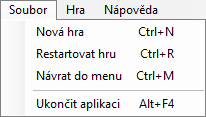
\includegraphics[width=0.3\textwidth]{Figures/PanelNastrojuSoubor.png}
	} 
	\hspace{3em} % make more space
	\subfloat[Nabídka hra\label{fig:PanelNastrojuHra}]
	{
		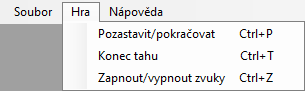
\includegraphics[width=0.45\textwidth]{Figures/PanelNastrojuHra2.png}
	} 
	\hspace{3em} % make more space
	\subfloat[Nabídka nápověda\label{fig:PanelNastrojuNapoveda}]
	{
		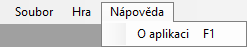
\includegraphics[width=0.4\textwidth]{Figures/PanelNastrojuNapoveda2.png}
	} 
	\caption{Dostupné nabídky panelu nástrojů}
	\label{fig:PanelNastroju}
\end{figure}

Každý hráč má přidělenou vlastní barvu, vzhledem k šesticípému rozložení herní desky je také přidělováno šest různých barev. Občas se ale některé kameny nebo pole od ostatních odlišují. Jeden z těchto případů nastává při zvýraznění kamene, tato situace je na příkladu zvýraznění kamene lidského hráče znázorněna na obrázku číslo \ref{fig:ZvyrazneniHracovaPole}. Ke zvýraznění kamene dochází u lidského a počítačového hráče z odlišných důvodů. U lidského hráče je znázorněn vždy ten kámen, na který uživatel jako poslední klikl. Díky tomuto zvýraznění je tedy uživateli jasné, se kterým kamenem právě manipuluje. U počítačového hráče dochází po konci tahu ke zvýraznění jím přesunutého kamene, díky čemuž je pak uživateli jasné, na jakou pozici se počítačový hráč během tahu posunul. Pro zvýraznění kamenů byly vytvořeny třídy, a to sice \lstinline$ZvyrazneniPoleLidskehoHrace$ a~\lstinline$ZvyrazneniPolePocitacovehoHrace$.

\begin{figure}
	\centering
	
\includegraphics[width=0.3\textwidth]{Figures/ZvyrazneniHracovaPole.png}
	\caption{Zvýraznění hráčova pole}
    \label{fig:ZvyrazneniHracovaPole}
\end{figure}

Kromě nové pozice kamene ale uživatele může zajímat také stará pozice kamene, tedy umístění kamene před provedením tahu. Z toho důvodu bylo potřeba vymyslet nějaký způsob, jakým uživatele informujeme o poloze kamenů před provedením tahu. Jako nejintuitivnější způsob k dosažení tohoto cíle bylo vybráno označení původní polohy kamene bledším odstínem barvy daných hráčů. V aplikaci má toto obarvení pole vlastní objekt, \lstinline$VychoziPolePocitacovehoHrace$, zde můžeme příklad označení původní polohy kamene pro každého počítačového hráče najít na obrázku číslo \ref{fig:VychoziPole}. Pole je tímto způsobem obarveno vždy pouze po dobu jednoho tahu, po provedení dalšího tahu už dané pole tímto způsobem označeno není.

\begin{figure}
	\centering
	\subfloat[Červený\label{fig:VychoziPoleCerveny}]
	{
		
\includegraphics[width=0.15\textwidth]{Figures/VychoziPoleCerveny.png}
	} 
	\hspace{1em} % make more space
	\subfloat[Zelený\label{fig:VychoziPoleZeleny}]
	{
		
\includegraphics[width=0.15\textwidth]{Figures/VychoziPoleZeleny.png}
	}
		\hspace{1em} % make more space
	\subfloat[Fialový\label{fig:VychoziPoleFialovy}]
	{
		
\includegraphics[width=0.15\textwidth]{Figures/VychoziPoleFialovy.png}
	}
		\hspace{1em} % make more space
	\subfloat[Hnědý\label{fig:VychoziPoleHnedy}]
	{
		
\includegraphics[width=0.15\textwidth]{Figures/VychoziPoleHnedy.png}
	}
		\hspace{1em} % make more space
	\subfloat[Žlutý\label{fig:VychoziPoleZluty}]
	{
		
\includegraphics[width=0.15\textwidth]{Figures/VychoziPoleZluty.png}
	}
	\caption{Vyznačení původní polohy kamene pro jednotlivé počítačové hráče}
	\label{fig:VychoziPole}
\end{figure}

\section{Komunikace mezi herním oknem a hrou}
Jak už bylo zmíněno v předchozí podkapitole, k vykreslování celé herní desky se všemi objekty dochází v metodě \lstinline$Paint$ prvku \lstinline$herniPanel$. Tuto metodu můžeme nalézt v třídě \lstinline$HraForm$. Samotná hra je ale vytvářena a spravována v jiné třídě, a to ve třídě \lstinline$Hra$. Je tedy nutné nějakým způsobem dostat údaje o aktuálním stavu hry ze třídy \lstinline$Hra$ do třídy \lstinline$HraForm$. Pro tyto účely je ve třídě \lstinline$Hra$ implementována klíčová metoda \lstinline$HerniPrvky$, jejíž návratovou hodnotou jsou kolekce všech objektů vyobrazovaných na herní desce (implementace této metody je znázorněna na výpisu \ref{src:metodaHerniPrvky}).

\begin{lstlisting}[label=src:metodaHerniPrvky,caption={Metoda vracející kolekce všech vyobrazovaných objektů}]
public (List<Pole>, List<LidskyHrac>, List<PocitacovyHrac>, List<MoznyTahLidskehoHrace>, ZvyrazneniPoleLidskehoHrace, List<ZvyrazneniPolePocitacovehoHrace>, List<VychoziPolePocitacovehoHrace>) HerniPrvky()
{
    return (herniPole, poleLidskehoHrace, polePocitacovehoHrace, mozneTahyLidskehoHrace, zvyrazneniPoleLidskehoHrace, zvyraznenaPolePocitacovehoHrace, vychoziPolePocitacovehoHrace);
}
\end{lstlisting}

V tuto chvíli máme sice ve třídě \lstinline$HraForm$ veškeré kolekce potřebné k vyobrazení celé herní desky, neznáme ale zatím žádný způsob, který by mohl být použit k vykreslení jednotlivých objektů. Z toho důvodu obsahuje každý objekt, který budeme chtít vykreslovat, metodu umožňující kreslení. Názorný příklad si ukážeme na kamenu lidského hráče. Jedním z argumentů události \lstinline$Paint$ prvku \lstinline$herniPanel$ je \lstinline$PaintEventArgs$ \cite{painteventargs}, což je třída sloužící k poskytování dat události \lstinline$Paint$. K vykreslení jednotlivých objektů pak stačí v daných objektech implementovat metodu, které předáme instanci třídy \lstinline$PaintEventArgs$. U kamene lidského hráče má tato metoda jméno \lstinline$NakresliLidskehoHrace$, přičemž v této metodě stačí pak využít instanci třídy ke kreslení a nakreslit útvar, s tím že barva a poloha tohoto útvaru závisí na parametrech daného objektu. V metodě \lstinline$Paint$ pak už jen stačí projít v cyklu všechny kolekce objektů získané pomocí metody \lstinline$HerniPrvky$, zavolat u všech objektů metody určené pro jejich vykreslování, a herní deska je z grafického hlediska hotová.

Pro lepší pochopení jsou ve výpisech \ref{src:metodaNakresliLidskehoHrace} a \ref{src:metodaIteraceKamenyHrace} obsaženy zmíněné metody a postupy.

\begin{lstlisting}[label=src:metodaNakresliLidskehoHrace,caption={Metoda vykreslující kámen lidského hráče}]
public void NakresliLidskehoHrace(PaintEventArgs e)
{
    e.Graphics.FillEllipse(br, this.poz_X_LHr, this.poz_Y_LHr, this.sirkaPole, this.vyskaPole);
    e.Graphics.DrawEllipse(pen, this.poz_X_LHr, this.poz_Y_LHr, this.sirkaPole, this.vyskaPole);
}
\end{lstlisting}

\newpage

\begin{lstlisting}[label=src:metodaIteraceKamenyHrace,caption={Metoda vykreslující postupně všechny kameny lidského hráče}]
foreach (LidskyHrac h in poleLidskehoHrace)
{
    h.NakresliLidskehoHrace(e);
}
\end{lstlisting}

Implementací těchto metod můžeme vykreslování herní desky považovat za vyřešené. Je ale ještě nutné vyřešit uživatelský vstup, tedy přesuny hráčových polí. Ve třídě \lstinline$HraForm$ zajišťuje zpracování uživatelského vstupu událost \lstinline$MouseClick$ prvku \lstinline$herniPanel$, která je vyvolána při každém kliknutí na panel. Z této metody pak voláme metodu \lstinline$PanelKliknuti$ třídy \lstinline$Hra$, které předáme přesné souřadnice uživatelova kliknutí. 

V této metodě je nejprve ověřeno, jestli uživatel vůbec klikl na nějaké herní pole. Pokud ano, je ověřeno, jestli se jedná o některý z jeho kamenů nebo možných tahů. Po ověření následuje provedení příslušného postupu, tyto postupy jsou detailněji popsány v podkapitole \ref{sec:VytvoreniMoznychTahu}. Po vykonání metody \lstinline$PanelKliknuti$ je potřeba uživatelovi zobrazit nový stav herní desky, proto je herní panel obnoven zavoláním metody \lstinline$Refresh$.


\section{Ostatní okna}
Aplikace obsahuje kromě herního okna několik dalších, převážně pomocných oken. Prvním oknem, které se uživateli zobrazí po spuštění aplikace, je hlavní menu (v aplikaci pod názvem \lstinline$MenuForm$, v~této práci obrázek číslo \ref{fig:HlavniMenu}). Kromě zobrazení banneru slouží ke snadnému a přímému přístupu ke všem částem aplikace.

Nyní projdeme zbývající okna postupně v pořadí, v jakém je tlačítko sloužící k jejich otevření umístěno v hlavním menu. Po kliknutí na tlačítko \textsf{Nová hra} je otevřeno okno ve kterém uživatel nastavuje parametry hry (v aplikaci pod názvem \lstinline$ParametryHryForm$, v této práci obrázek číslo \ref{fig:ParametryHry}). V tomto okně si uživatel navolí počet počítačových hráčů, proti kterým bude hrát, jejich obtížnost, a také kdo bude první na tahu. Jediným omezením je, že uživatel musí vždy vybrat některou z~nabízených možností, pokud se pokusí vytvořit hru bez nastavení počtu hráčů nebo začínajícího hráče, je mu zobrazeno dialogové okno s chybovou hláškou.

\begin{figure}
	\centering
	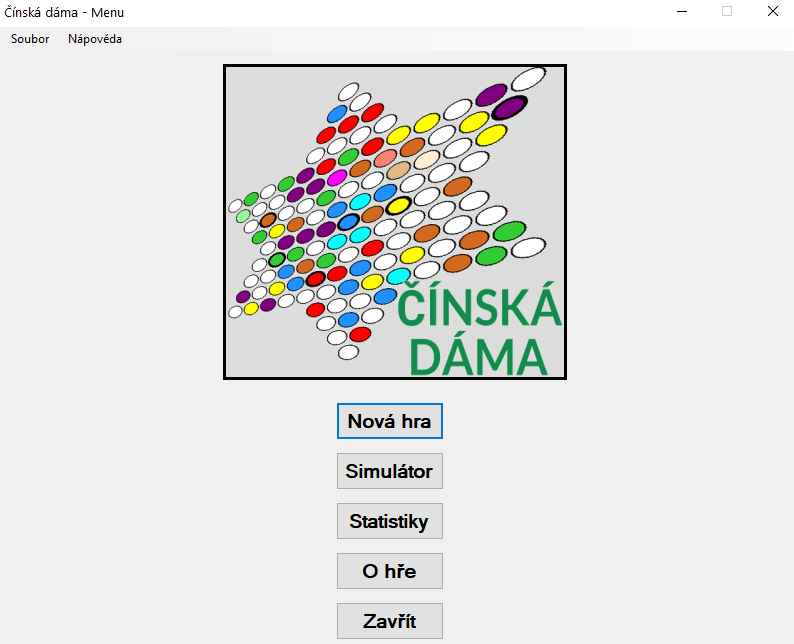
\includegraphics[width=0.6\textwidth]{Figures/HlavniMenu.png}
	\caption{Okno \textsf{Hlavní menu}}
    \label{fig:HlavniMenu}
\end{figure}

\begin{figure}
	\centering
	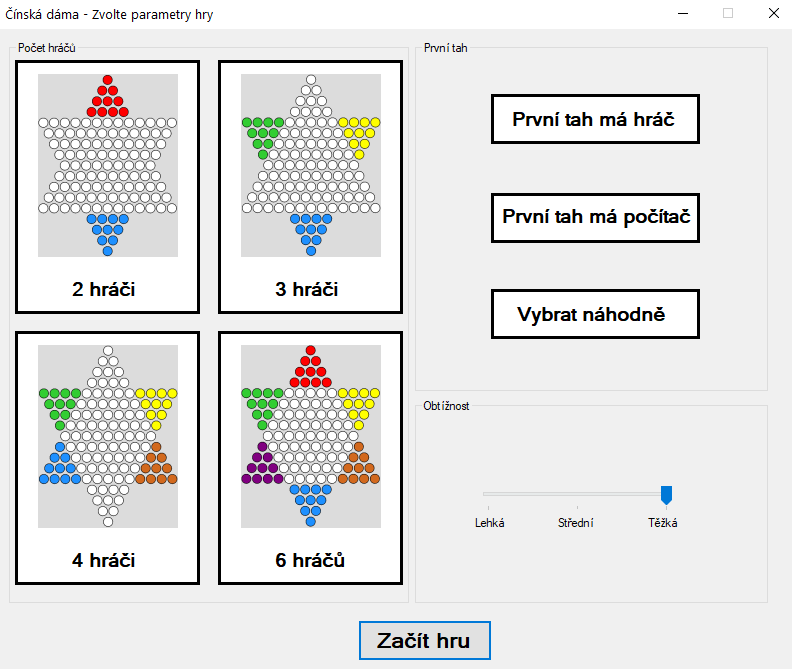
\includegraphics[width=0.6\textwidth]{Figures/ParametryHry.png}
	\caption{Okno \textsf{Parametry hry}}
    \label{fig:ParametryHry}
\end{figure}

Na stejném principu funguje i další okno, které se zobrazí po kliknutí na tlačítko \textsf{Simulátor}. Jedná se o okno, ve kterém uživatel nastavuje parametry simulátoru (v aplikaci pod názvem \lstinline$ParametrySimulatoruForm$, v této práci obrázek číslo \ref{fig:ParametrySimulatoru}). Hráč zde před spuštěním simulace zvolí počet počítačových hráčů hrajících v dané simulaci a také jejich obtížnost. Okno je navrženo s ohledem na co největší srozumitelnost, po výběru určitého počtu hráčů je vždy zobrazena herní deska s odpovídajícím rozvržením k danému počtu hráčů, a obtížnosti jednotlivých hráčů jsou umístěny na místech, kde by se nacházeli skuteční hráči při hře s využitím fyzické desky.

\begin{figure}
	\centering
	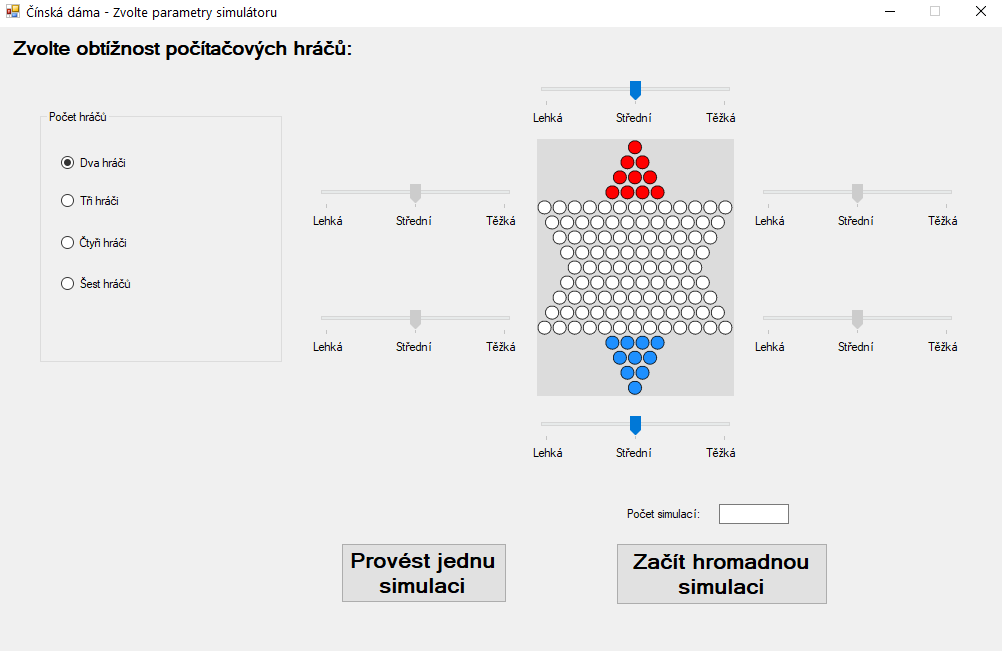
\includegraphics[width=0.6\textwidth]{Figures/ParametrySimulatoru.png}
	\caption{Okno \textsf{Parametry simulátoru}}
    \label{fig:ParametrySimulatoru}
\end{figure}
Dalším oknem nacházejícím se v aplikaci je okno se statistikami (v aplikaci jej najdeme pod názvem \lstinline$StatistikyForm$, v této práci obrázek číslo \ref{fig:Statistiky}). Jeho účelem je poskytnutí uživatelsky srozumitelné interpretace souboru \textsf{Statistiky.txt}, který obsahuje záznamy o všech provedených simulacích. Jak napovídá text uvedený v samotném okně, okno neslouží k zaznamenávání her lidského hráče. zaznamenávány jsou zde pouze výsledky simulací.

\begin{figure}
	\centering
	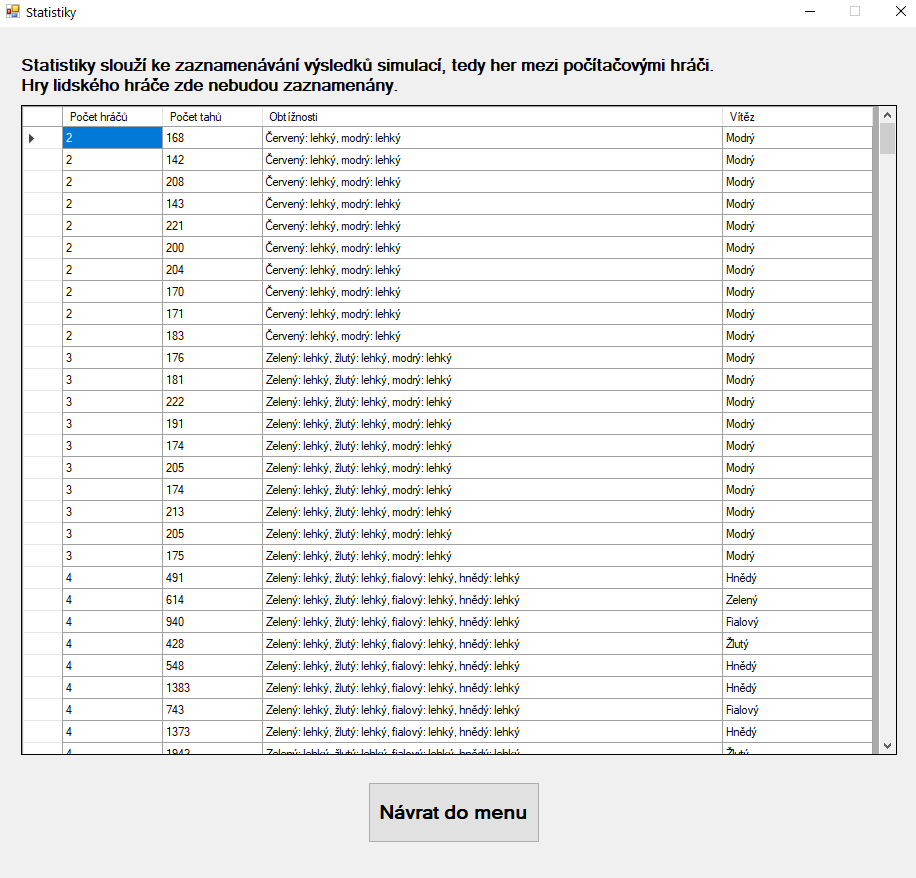
\includegraphics[width=0.6\textwidth]{Figures/Statistiky.png}
	\caption{Okno \textsf{Statistiky}}
    \label{fig:Statistiky}
\end{figure}

Posledním oknem je okno \textsf{O hře} (v aplikaci pod názvem \lstinline$InformaceForm$, v této práci obrázek číslo \ref{fig:OHre}). Otevřít jej lze dvěma způsoby. Jednak po výběru možnosti \textsf{O hře} v hlavním menu, a~jednak po výběru možnosti \textsf{Nápověda}, která je k dispozici v panelu nástrojů při hře. Okno obsahuje základní informace týkající se pravidel a ovládání hry, které by mohly novému uživateli pomoci v~pochopení hry. Kromě toho je zde také krátká zmínka o autorovi aplikace a o účelu jejího vytvoření.

\begin{figure}
	\centering
	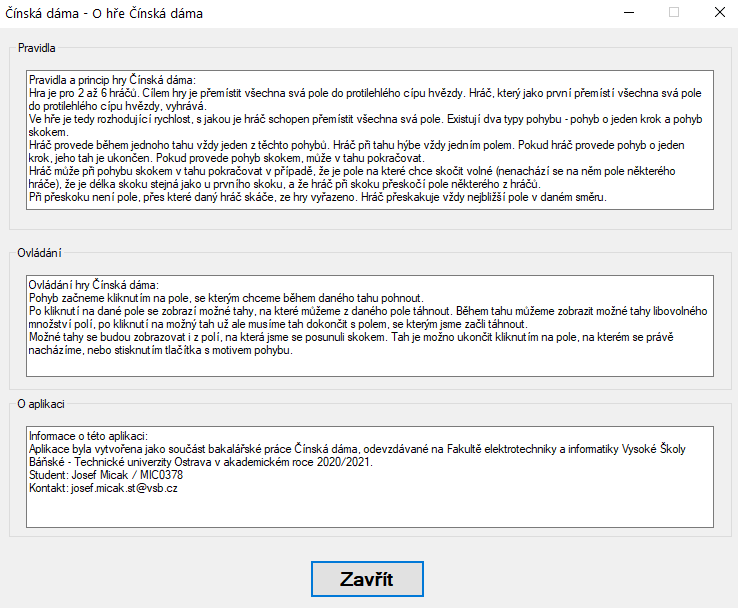
\includegraphics[width=0.6\textwidth]{Figures/OHre.png}
	\caption{Okno \textsf{O hře}}
    \label{fig:OHre}
\end{figure}
\endinput
\chapter{Analýza odehraných her}
\section{Hry mezi lidským a počítačovým hráčem}
Práce neobsahuje podrobnou analýzu odebraných her lidského hráče proti jednomu nebo více počítačových hráčů, a to kvůli tomu, že taková analýza by byla silně závislá na dovednosti a momentálním rozpoložení lidského hráče. Z toho důvodu bychom takovou analýzu nemohli považovat za objektivní a směrodatnou. Proto analyzujeme hlavně vzájemné hry počítačových hráčů, ti totiž nejsou ovlivňováni externími vlivy a jejich dovednosti jsou jasně definované (viz podkapitola \ref{sec:UrovneObtiznosti}). Tento způsob analýzy lze tedy považovat za objektivní, samotnou analýzu lze najít v následující podkapitole.

I přesto lze ale určit, jak hra vzhledem k dovednosti lidského hráče pravděpodobně dopadne. Lehkému počítačovému hráči bychom také mohli přidělit název \enquote{pasivní}, jeho postup totiž není příliš rychlý a dokončení hry trvá zejména u hráčů začínajících v jiných než nejvýše a nejníže položeném trojúhelníku mimořádně dlouhou dobu. Dá se tedy říct, že hra proti lehkému hráči by neměla být příliš velká výzva ani pro úplného začátečníka, který se pouze seznamuje s principy hry.

Následuje střední hráč. Ten by už mohl být začátečníkovi rovnocenným soupeřem, pro mírně pokročilého už ale opět nebude představovat příliš velkou výzvu, takový lidský hráč by jej měl bez problému porazit.

Posledním zbývajícím počítačovým hráčem je těžký hráč. Ten už je vzhledem ke všem implementovaným funkcím a kontrolám rovnocenným soupeřem i pro pokročilého hráče. Hra v takovém případě končí většinou výhrou některého z hráčů o několik tahů. Je ale nutné brát v potaz funkci, která kontroluje, jestli provedení daného tahu počítačového hráče neumožní lidskému hráči provedení pro něj výhodnějšího tahu než předtím. Tato funkce je totiž u tohoto hráče využívána, z čehož vyplývá, že síla tohoto hráče spočívá mimo jiné v jeho počtu. U hry jednoho lidského hráče proti pěti počítačovým hráčům je totiž při každém tahu každého počítačového hráče kontrolováno, jestli provedení tahu nezvýhodní lidského hráče. U hry dvou hráčů není tato funkce vzhledem k menšímu počtu kamenů na herní desce příliš důležitá, u hry šesti hráčů ale velmi výrazně ztíží lidskému hráči přesun ke svému cílovému trojúhelníku. Vyhrát proti pěti počítačovým hráčům s obtížností těžký je tudíž podstatně těžší než vyhrát proti jednomu hráči s toutéž obtížností. Může se tedy stát, že hráč, který stabilně poráží jednoho počítačového hráče s obtížností těžký, nebude schopen porazit vyšší počet počítačových hráčů s touto obtížností.

\section{Hry mezi počítačovými hráči}
\label{sec:HryMeziPocitacovymiHraci}
V této práci budou dovednosti jednotlivých počítačových hráčů prezentovány dvěma způsoby. Prvním je průměrný počet tahů potřebných k výhře u her počítačových hráčů stejné obtížnosti. Tyto výsledky jsou uvedeny v tabulce \ref{tab:PocetTahuStejniHraci}.

\begin{table}
	\centering
	\caption{Průměrný počet tahů potřebných k výhře počítačových hráčů podle jejich obtížností}
	\label{tab:PocetTahuStejniHraci}
	\begin{tabular}{cd{5}d{5}d{5}d{5}d{5}}
		\toprule
		Obtížnost hráčů & \multicolumn{1}{c}{Dva hráči} & \multicolumn{1}{c}{Tři hráči} & \multicolumn{1}{c}{Čtyři hráči} & \multicolumn{1}{c}{Šest hráčů} & \multicolumn{1}{c}{Průměr}\\
		\midrule
		Lehký & 164,2 & 200,1 & 1106,3 & 233,8 & 426,1\\
		Střední & 93,4 & 88,1 & 85,7 & 89,3 & 89,1\\
		Těžký & 35 & 34 & 31 & 35 & 33,7\\
		\bottomrule
	\end{tabular}
    \begin{tablenotes}
      \small
      \item *U hráče jsou sice výsledky zprůměrovány z 50 her, výsledky her jsou nicméně z důvodu absence náhodných tahů ve všech případech totožné
    \end{tablenotes}
\end{table}

Z údajů v posledním sloupci tabulky můžeme vyčíst, že střední hráč dokončí hru jednoznačně rychleji než lehký hráč, a stejně tak těžký hráč dokončí hru jednoznačně rychleji než střední hráč. Z~toho vyplývá, že mezi hráči jsou očividné dovednostní rozdíly a že jsou jednotliví hráči implementováni korektně, jinak řečeno, nestává se, že například lehký hráč dokončí hru rychleji než střední hráč.

Druhým způsobem prezentace dovedností jednotlivých hráčů je analýza výsledků her, ve kterých proti sobě hrají hráči různých obtížností. Vzhledem k velmi vysokému počtů kombinací her s ohledem na počet hráčů a jejich obtížnosti analyzujeme hry vždy jednoho počítačového hráče vyšší obtížnosti s počítačovými hráči menší obtížnosti. Například u hry šesti hráčů, viz tabulka \ref{tab:TurnajSestHracu}, nastoupí proti sobě jeden počítačový hráč těžší obtížnosti a pět počítačových hráčů lehčí obtížnosti. Poloha těžšího počítačového hráče se mění, vždy je analyzováno 50 her pro každý možný výchozí trojúhelník počítačového hráče s vyšší obtížností. Za předpokladu že dříve, než počítačový hráč vyšší obtížnosti dokončí hru libovolný hráč nižší obtížnosti, je hra v tabulce zapsána ve prospěch hráče s nižší obtížností.

\begin{table}
	\centering
	\caption{Turnaj hráčů různých obtížností ve hře pro dva hráče}
	\label{tab:TurnajDvaHraci}
	\begin{tabular}{cccc}
		\toprule
		Obtížnost hráčů & \multicolumn{1}{c}{Lehký} & \multicolumn{1}{c}{Střední} & \multicolumn{1}{c}{Těžký}\\
		\midrule
		Lehký & \faTimes & 3 : 97 & 0 : 100\\
		Střední & 97 : 3 & \faTimes & 0 : 100\\
		Těžký & 100 : 0 & 100 : 0 & \faTimes\\
		\bottomrule
	\end{tabular}
\end{table}

\begin{table}
	\centering
	\caption[Turnaj hráčů různých obtížností ve hře pro tři hráče]{Turnaj hráčů různých obtížností ve hře pro tři hráče -- údaj 5: 145 uvedený v prvním řádku druhého sloupce znamená, že ze 150 proběhlých her (50 pro každý možný výchozí trojúhelník hráče s vyšší obtížností) 5$\times$ vyhrál některý ze dvou hráčů lehké obtížnosti a 145$\times$ vyhrál hráč střední obtížnosti.}
	\label{tab:TurnajTriHraci}
	\begin{tabular}{cccc}
		\toprule
		Obtížnost hráčů & \multicolumn{1}{c}{Lehký} & \multicolumn{1}{c}{Střední} & \multicolumn{1}{c}{Těžký}\\
		\midrule
		Lehký & \faTimes & 5 : 145 & 2 : 148\\
		Střední & 145 : 5 & \faTimes & 2 : 148\\
		Těžký & 148 : 2 & 148 : 2 & \faTimes\\
		\bottomrule
	\end{tabular}
\end{table}

\begin{table}
	\centering
	\caption{Turnaj hráčů různých obtížností ve hře pro čtyři hráče}
	\label{tab:TurnajCtyriHraci}
	\begin{tabular}{cccc}
		\toprule
		Obtížnost hráčů & \multicolumn{1}{c}{Lehký} & \multicolumn{1}{c}{Střední} & \multicolumn{1}{c}{Těžký}\\
		\midrule
		Lehký & \faTimes & 0 : 200 & 0 : 200\\
		Střední & 200 : 0 & \faTimes & 24 : 176\\
		Těžký & 200 : 0 & 176 : 24 & \faTimes\\
		\bottomrule
	\end{tabular}
\end{table}

\begin{table}
	\centering
	\caption{Turnaj hráčů různých obtížností ve hře pro šest hráčů}
	\label{tab:TurnajSestHracu}
	\begin{tabular}{cccc}
		\toprule
		Obtížnost hráčů & \multicolumn{1}{c}{Lehký} & \multicolumn{1}{c}{Střední} & \multicolumn{1}{c}{Těžký}\\
		\midrule
		Lehký & \faTimes & 8 : 292 & 6 : 294\\
		Střední & 292 : 8 & \faTimes & 40 : 260\\
		Těžký & 294 : 6 & 260 : 40 & \faTimes\\
		\bottomrule
	\end{tabular}
\end{table}

\begin{table}
	\centering
	\caption{Turnaj hráčů různých obtížností -- souhrn všech her}
	\label{tab:TurnajSouhrn}
	\begin{tabular}{cccc}
		\toprule
		Obtížnost hráčů & \multicolumn{1}{c}{Lehký} & \multicolumn{1}{c}{Střední} & \multicolumn{1}{c}{Těžký}\\
		\midrule
		Lehký & \faTimes & 2,2 \% & 0,8 \%\\
		Střední & 97,7 \% & \faTimes & 7,5 \%\\
		Těžký & 99,1 \% & 92,4 \% & \faTimes\\
		\bottomrule
	\end{tabular}
\end{table}

Vzhledem k podmínce, že je na herní desce jeden hráč vyšší obtížnosti a zbývající rohy obsadí hráči nižší obtížnosti, logicky se stoupajícím počtem hráčů stoupá počet analyzovaných her, protože určený počet 50 her je pevný a neměnný. V souhrnné tabulce proto neuvádíme, kolik her z celkového počtu her daný hráč vyhrál, nýbrž u každé z tabulek zaznamenáme podíl her, které daný hráč vyhrál, a z těchto podílů pak spočítáme průměr, který ve výsledku uvedeme v souhrnné tabulce. Tím je zajištěno, že hry dvou hráčů mají na údaje uvedené v souhrnné tabulce stejný vliv jako hry šesti hráčů, a to i přestože je jich v absolutních číslech třikrát méně.

V tabulkách \ref{tab:TurnajDvaHraci}, \ref{tab:TurnajTriHraci}, \ref{tab:TurnajCtyriHraci}, \ref{tab:TurnajSestHracu} a souhrnné tabulce \ref{tab:TurnajSouhrn} můžeme vidět statistiky výsledků her počítačových hráčů různých obtížností. Z výsledků lze usoudit, že hry dopadly podle očekávání, ve většině případů vyhrál počítačový hráč vyšší obtížnosti. V některých případech vyhrál počítačový hráč nižší obtížnosti, k čemuž mohlo dojít například \enquote{zapomenutím} některého z kamenů hráče vyšší obtížnosti na kraji herní desky nebo rychlým postupem jiného hráče směrem na pole, která jsou umístěna před cílovým trojúhelníkem hráče vyšší obtížnosti, což ve výsledku výrazně zpomalí postup hráče vyšší obtížnosti.

Detailní záznamy o všech odehraných hrách analyzovaných v této podkapitole jsou, stejně jako jakékoli další simulace provedené uživatelem, uloženy ve statistikách ke kterým lze přistoupit přes hlavní menu. 
\endinput
\chapter{Závěr}
Cílem této bakalářské práce bylo popsat pravidla a principy deskové hry Čínská dáma a následně provést implementaci umožňující uživateli hru proti jednomu nebo více počítačovým hráčům. 

Všechny cíle bakalářské práce byly splněny, první část práce podrobně popisuje základní principy této deskové hry a také poukazuje na značnou nejednotnost co se týče pravidel hry, přičemž vysvětluje, s využitím kterých konkrétních pravidel je počítáno v rámci této práce. Další části práce poté mimo jiné vysvětlují zvolené postupy při implementaci jednotlivých částí a prvků hry. Uživatel si může při vytváření hry kromě počtu počítačových hráčů, proti kterým bude hrát, zvolit také jejich obtížnost. Na výběr je z celkem tří různých obtížností, dovednosti jednotlivých počítačových hráčů podle jejich obtížnosti jsou pak prakticky porovnávány v poslední části, ve které je na základě více kritérií zanalyzováno větší množství her mezi počítačovými hráči stejných i různých obtížností.

Mezi možná vylepšení nebo rozšíření vytvořené aplikace bychom mohli zařadit možnost začínat v jiném trojúhelníku na herní desce nebo vlastní výběr barev jednotlivých hráčů, v této práci jsou barvy neměnné zejména z důvodu usnadnění odlišitelnosti různých hráčů. Dále by uživatel mohl mít možnost vybrat si vlastní interpretaci pravidel, někteří uživatele by totiž mohli preferovat ovládání více sad kamenů najednou nebo povolení tahů do všech polí na herní desce. V neposlední řadě také existuje prostor pro vylepšení dovedností počítačového hráče s nejvyšší obtížností, ačkoli by v~takovém případě vzniklo riziko, že u her s více počítačovými hráči s touto obtížností by pak výpočet jejich tahů trval příliš dlouhou dobu.

\hfill Josef Micak
\endinput

\appendix
\chapter{Projekt}
Příloha slouží pro splnění části požadavků projektu ze předmětu Elektronické publikování.

\textbf{Zvýrazněný text}.

\begin{comment}
  \section{Zakomentovaná sekce}
  Obsah zakomentované sekce
\end{comment}

Graf výkonnosti pracovníka během 8hodinového pracovního dne:

\begin{gnuplot}[terminal=pdf,terminaloptions=color]
    unset key
    set samples 10000
    set format '%g'
    set xlabel "Počet odpracovaných hodin"
    set ylabel "Výkonnost"
    set xrange [0:8]
    set yrange [0:1]
    plot sin((x/3.35)+0.75)
\end{gnuplot}

\begin{figure}
  \begin{center}
  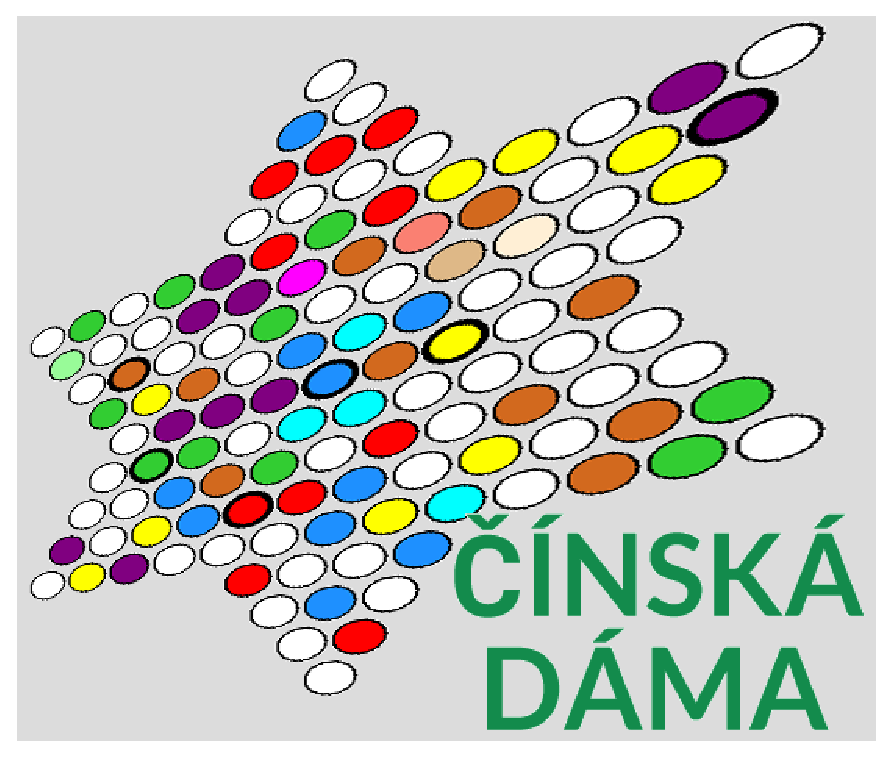
\includegraphics[scale=0.5, angle=15]{Figures/ExampleObrazek.eps}
  \caption{Obrázek vložený prostředím \texttt{graphicx}.}
  \label{obr.graphicx}
  \end{center}
\end{figure}

\begin{music}
\parindent10mm
\instrumentnumber{1}       
\setname1{Piano}           
\setstaffs1{2}             
\generalmeter{\meterfrac44}
\startextract             
\Notes\ibu0f0\qb0{cge}\tbu0\qb0g|\hl j\en
\Notes\ibu0f0\qb0{cge}\tbu0\qb0g|\ql l\sk\ql n\en
\bar
\Notes\ibu0f0\qb0{dgf}|\qlp i\en
\notes\tbu0\qb0g|\ibbl1j3\qb1j\tbl1\qb1k\en
\Notes\ibu0f0\qb0{cge}\tbu0\qb0g|\hl j\en\endextract                
\end{music}

{\fontfamily{pcr}\selectfont
Font Courier
}

{\fontfamily{lmdh}\selectfont
Font Latin Modern Dunhill
}



\endinput

\let\addspace\biblatexaddspace
\printbibliography[title={Literatura}, heading=bibintoc]

\printindex
\end{document}
